% =====================================================================
%  Mobility internship report -- Abdelwahab LAKSIRI
%  LAMMOC, Universidade Federal Fluminense (UFF)
%  Compile:  latexmk -pdf report.tex      (or pdflatex twice)
% =====================================================================
\documentclass[11pt,a4paper,oneside]{report}

% ---------------------------------------------------------------------
%  Edit these before submitting -- they were left as placeholders on
%  purpose rather than guessed.
% ---------------------------------------------------------------------
\newcommand{\InternshipPeriod}{June 2026 -- September 2026}
\newcommand{\ReportDate}{27/09/2026}
\newcommand{\Programme}{\ Industrial Management}

% ---------------------------------------------------------------------
\usepackage[T1]{fontenc}
\usepackage[utf8]{inputenc}
\usepackage{lmodern}
\usepackage{microtype}
\usepackage[margin=2.5cm,headheight=14pt]{geometry}
\usepackage{graphicx}
\usepackage{booktabs}
\usepackage{tabularx}
\usepackage{array}
\usepackage{multirow}
\usepackage{makecell}
\usepackage{amsmath,amssymb}
\usepackage[dvipsnames,table]{xcolor}
\usepackage{float}
\usepackage{caption}
\usepackage{subcaption}
\usepackage{enumitem}
\usepackage{setspace}
\usepackage{fancyhdr}
\usepackage{titlesec}
\usepackage{csquotes}
\usepackage[most]{tcolorbox}
\usepackage{tikz}
\usetikzlibrary{positioning,arrows.meta,shapes.geometric,calc}
\usepackage[hidelinks]{hyperref}

\setstretch{1.12}
\setlength{\parskip}{0.45em}
\setlength{\parindent}{0pt}
\setlist{itemsep=0.2em,topsep=0.3em}
\captionsetup{font=small,labelfont=bf,margin=0.5cm}
\graphicspath{{figures/}}

% ---------- colours ----------
\definecolor{fire}{HTML}{D84315}
\definecolor{goes}{HTML}{1565C0}
\definecolor{inpe}{HTML}{6A5F7A}
\definecolor{good}{HTML}{2E7D32}
\definecolor{ink}{HTML}{222222}
\definecolor{soft}{HTML}{F4F6F8}

% ---------- chapter style ----------
\titleformat{\chapter}[display]
  {\normalfont\bfseries\color{ink}}
  {\color{fire}\large\mdseries\scshape Chapter \thechapter}
  {0.4em}
  {\Huge}
  [\vspace{0.2em}{\color{fire}\titlerule[1.2pt]}]
\titlespacing*{\chapter}{0pt}{-10pt}{22pt}
\titleformat{\section}{\normalfont\Large\bfseries\color{ink}}{\thesection}{0.8em}{}
\titleformat{\subsection}{\normalfont\large\bfseries\color{ink}}{\thesubsection}{0.8em}{}

% ---------- header / footer ----------
\pagestyle{fancy}
\fancyhf{}
\fancyhead[L]{\small\color{gray}Wildfire prediction in the Pantanal}
\fancyhead[R]{\small\color{gray}A.~LAKSIRI -- LAMMOC/UFF}
\fancyfoot[C]{\thepage}
\renewcommand{\headrulewidth}{0.3pt}
\fancypagestyle{plain}{\fancyhf{}\fancyfoot[C]{\thepage}\renewcommand{\headrulewidth}{0pt}}

% ---------- boxes ----------
\newtcolorbox{plainbox}[1][In plain words]{
  enhanced, colback=soft, colframe=goes!70!black, boxrule=0.6pt,
  arc=2pt, left=8pt, right=8pt, top=6pt, bottom=6pt,
  fonttitle=\bfseries\small, coltitle=white, colbacktitle=goes!80!black,
  title={#1}}
\newtcolorbox{keybox}[1][Key result]{
  enhanced, colback=good!6, colframe=good!70!black, boxrule=0.6pt,
  arc=2pt, left=8pt, right=8pt, top=6pt, bottom=6pt,
  fonttitle=\bfseries\small, coltitle=white, colbacktitle=good!75!black,
  title={#1}}
\newtcolorbox{warnbox}[1][Pitfall found and fixed]{
  enhanced, colback=fire!5, colframe=fire!75!black, boxrule=0.6pt,
  arc=2pt, left=8pt, right=8pt, top=6pt, bottom=6pt,
  fonttitle=\bfseries\small, coltitle=white, colbacktitle=fire!80!black,
  title={#1}}

\newcommand{\code}[1]{\texttt{\small #1}}
\newcommand{\sig}{\ensuremath{\sigma}}

% =====================================================================
\begin{document}

% ============================ TITLE PAGE =============================
\begin{titlepage}
\newgeometry{margin=2.2cm}
\centering
{\large\scshape Université Mohammed VI Polytechnique (UM6P)\par}
{\large EMINES -- School of Industrial Management\par}
\vspace{0.3cm}
{\color{fire}\rule{\linewidth}{1.2pt}\par}
\vspace{0.9cm}
{\Large\scshape Mobility Internship Report\par}
\vspace{1.0cm}
{\huge\bfseries\color{ink}
Predicting Wildfire Persistence, Spread\\[0.25em]
and Ignition in the Pantanal\\[0.25em]
with Satellite Data and Machine Learning\par}
\vspace{0.7cm}
{\large\itshape From a once-a-day forecast to an hour-by-hour one,\\
and what the weather really controls\par}
\vspace{1.4cm}

\begin{tabular}{rl}
\textbf{Author:}      & Abdelwahab \textsc{LAKSIRI} \\[0.3em]
\textbf{Supervisor:}  & Prof.\ Marcio \textsc{CATALDI} \\[0.3em]
\textbf{Host laboratory:} & LAMMOC -- Climate System Monitoring and Modeling Laboratory \\
                      & Universidade Federal Fluminense (UFF), Rio de Janeiro, Brazil \\[0.3em]
\textbf{Home institution:} & EMINES -- School of Industrial Management \\
                      & Université Mohammed VI Polytechnique (UM6P), Morocco \\[0.3em]
\textbf{Programme:}   & \Programme \\[0.3em]
\textbf{Period:}      & \InternshipPeriod \\
\end{tabular}

\vfill

\begin{tikzpicture}
  \foreach \i/\c in {0/goes,1/goes!70,2/good,3/fire!70,4/fire}{
    \fill[\c] (\i*1.1,0) rectangle ++(0.9,0.22);}
\end{tikzpicture}\par
\vspace{0.4cm}
{\large \ReportDate\par}
\restoregeometry
\end{titlepage}

% ============================ FRONT MATTER ===========================
\pagenumbering{roman}

\chapter*{Acknowledgements}
\addcontentsline{toc}{chapter}{Acknowledgements}

I would like to thank my supervisor, \textbf{Prof.\ Marcio CATALDI}, for
welcoming me into LAMMOC, for proposing this subject, and for pushing the work
towards the question that turned out to matter most: \emph{show me the model and
show me the scores}. His meteorological perspective shaped how every result in
this report is interpreted.

I thank the members of \textbf{LAMMOC} and the \textbf{Universidade Federal
Fluminense} for their hospitality and for the data they made available, in
particular the daily fire model that served as this project's starting point
and the Extreme Heatwave Index (XHWI) produced within the RiskClima project.

I also thank \textbf{EMINES -- School of Industrial Management} and
\textbf{Université Mohammed VI Polytechnique} for making this mobility
internship possible, and the teaching staff whose courses in statistics,
optimisation and data analysis I drew on throughout.

Finally, this work relies on openly available public data: the Programa
Queimadas of Brazil's National Institute for Space Research (INPE), the GOES-16
satellite products distributed by the U.S.\ National Oceanic and Atmospheric
Administration (NOAA), and the ERA5 reanalysis from the Copernicus Climate
Change Service (ECMWF). None of the analysis would have been possible without
them.

% ---------------------------------------------------------------------
\chapter*{Abstract}
\addcontentsline{toc}{chapter}{Abstract}

The Pantanal, the world's largest tropical wetland, has suffered some of the
most severe fire seasons on record in recent years, notably in 2020 and 2024.
The laboratory already had a machine-learning model that predicted, \emph{once
per day}, whether a fire would still be burning the next day and whether it
would spread. The goal of this internship was to build an \emph{hourly} version
of that model and to find out how much the weather actually contributes to the
predictions.

The work proceeded in four stages. \textbf{(1)} Reviewing the existing daily
model showed that its headline score (ROC-AUC 0.93 for persistence) was mostly
an artefact of how its table was filtered: a one-line rule with no model at all
scored 0.905. \textbf{(2)} An hourly-\emph{forcing} model was built from INPE
fire detections for 2019--2024 combined with hourly ERA5 weather. It reaches
ROC-AUC 0.67 for next-day persistence, and hourly wind gives a statistically
real improvement. However, the INPE satellite passes over the Pantanal only once
a day, so no truly hourly target can be built from it. \textbf{(3)} The
geostationary satellite GOES-16, which observes the region every 10 minutes,
was therefore brought in, its fire detections were validated against INPE (78\%
agreement, about 8 times better than chance), and a genuinely hourly model was
trained for 2024. \textbf{(4)} Physical checks showed that the first
\enquote{spread} target, defined on 28\,km weather-grid cells, was not measuring
spread at all (it implied a fire front moving at 7.7\,m/s). Fire was therefore
stored at the satellite's native 2\,km resolution and the target split into two
separate questions: \emph{spread} into adjacent ground and \emph{ignition} of new
fires nearby.

The final hourly models score ROC-AUC 0.83 (will the fire still burn in one
hour?), 0.81 (will a new fire start nearby?) and 0.75 (will the fire spread to
adjacent 2\,km ground?), against 0.5 for guessing. A paired statistical test
across five monthly evaluation folds shows that \textbf{weather improves only
the spread forecast} (+0.012 PR-AUC, $t=3.76$, $p=0.020$, 5 of 5 folds), while it
adds nothing measurable to persistence ($p=0.99$) or ignition ($p=0.89$). This
matches physics: persistence over one hour is governed by what the fire is
already doing, spread is driven by wind and dryness, and ignition in the
Pantanal follows the location of existing (largely human-set) fire activity.

The report is written for readers without a data-science background: every
technical idea is introduced in plain language before it is used.

\medskip
\textbf{Keywords:} wildfire, Pantanal, GOES-16, INPE, ERA5, machine learning,
XGBoost, random forest, fire spread, statistical significance.

% ---------------------------------------------------------------------
\tableofcontents
\listoffigures
\listoftables

\cleardoublepage
\pagenumbering{arabic}

% =====================================================================
\chapter{Introduction}
% =====================================================================

\section{Why fire in the Pantanal matters}

The \textbf{Pantanal} is the largest tropical wetland on Earth. It lies in the
centre of South America, mostly in the Brazilian states of Mato Grosso and Mato
Grosso do Sul, and extends into Bolivia and Paraguay. For part of the year large
areas are flooded; in the dry season (roughly June to October) the vegetation
dries out and becomes highly flammable. Most fires there are started by people
-- to clear land or renew pasture -- and then escape, helped by heat, low
humidity and wind.

In recent years the Pantanal has had exceptional fire seasons. In \textbf{2020} a
very large fraction of the Brazilian Pantanal burned, and \textbf{2024} was again
a severe year. Fire destroys habitat, kills wildlife, damages the health of
people exposed to smoke, and releases carbon. Anticipating \emph{which} fires
will keep burning, and \emph{where} fire will move next, helps decide where to
send limited firefighting resources.

\section{The host laboratory}

The internship took place at \textbf{LAMMOC} (Laboratório de Monitoramento e
Modelagem do Sistema Climático -- the Climate System Monitoring and Modeling
Laboratory) of the \textbf{Universidade Federal Fluminense (UFF)} in the state of
Rio de Janeiro, Brazil, under the supervision of \textbf{Prof.\ Marcio CATALDI}.
The laboratory works on climate monitoring and modelling, including extreme
events such as heatwaves; within the RiskClima project it produced the
\emph{Extreme Heatwave Index} (XHWI) used in this work.

This was a \textbf{mobility internship} of EMINES -- School of Industrial
Management, Université Mohammed VI Polytechnique (UM6P).

\section{Starting point and objectives}

The laboratory already had a \textbf{daily} fire model (notebook
\code{ml\_persist\_propaga\_wind.ipynb}). For every fire detected by satellite on
a given day, it predicted two things for the next day:
\begin{itemize}
  \item \textbf{persistence} -- will this fire still be burning tomorrow?
  \item \textbf{propagation (spread)} -- will fire appear in the area around it?
\end{itemize}

The objectives of the internship were:
\begin{enumerate}
  \item build an \textbf{hourly} version of this model for the Pantanal, using
        hourly weather data instead of daily averages;
  \item evaluate the models honestly, so that the scores can be trusted;
  \item answer a scientific question that came up repeatedly during the work:
        \textbf{how much does the weather actually matter} for predicting fire
        behaviour, and for which kind of behaviour?
\end{enumerate}

\section{What this internship produced}

\begin{itemize}
  \item A critical review of the existing daily model, showing that its headline
        persistence score was largely a data-filtering artefact
        (Section~\ref{sec:daily-artifact}).
  \item An hourly-forcing model based on INPE detections and ERA5 weather,
        2019--2024, with a rigorous test of which inputs really help
        (Chapter~\ref{ch:inpe}).
  \item A complete pipeline that reads the GOES-16 geostationary fire product,
        validated against INPE, giving a genuinely hourly fire record
        (Chapter~\ref{ch:goes}).
  \item A physically correct definition of fire \emph{spread} at 2\,km
        resolution, separated from the \emph{ignition} of new fires
        (Chapter~\ref{ch:spread}).
  \item Five trained models with measured skill, and a statistically tested
        answer to the question of where weather matters
        (Chapter~\ref{ch:results}).
  \item About a dozen data problems that would each have silently corrupted the
        results, found and fixed along the way (collected in
        Table~\ref{tab:bugs}).
\end{itemize}

\section{How to read this report}

Chapter~\ref{ch:concepts} explains, without assuming any background, the
concepts needed to follow the rest: how satellites see fire, what machine
learning is, and how one judges whether a model is good. Readers already familiar
with these can skip it. Chapter~\ref{ch:data} presents the study area and the
data. Chapter~\ref{ch:method} gives the overall plan, and
Chapters~\ref{ch:inpe}--\ref{ch:spread} follow the project in the order it was
done. Chapter~\ref{ch:results} collects the results and discusses the role of
weather, Chapter~\ref{ch:limits} lists the limitations, and
Chapter~\ref{ch:conclusion} concludes. Throughout, three kinds of boxes are used:

\begin{plainbox}
Blue boxes restate a technical idea in everyday language.
\end{plainbox}
\begin{keybox}
Green boxes highlight a main finding.
\end{keybox}
\begin{warnbox}
Red boxes describe a problem that was found in the data or code, why it
mattered, and how it was fixed.
\end{warnbox}

% =====================================================================
\chapter{Key concepts for non-specialists}\label{ch:concepts}
% =====================================================================

This chapter introduces every idea used later. It is deliberately
non-mathematical.

\section{How satellites see fire}

Fires are hot, and hot objects emit strongly in the \emph{infrared}. Satellite
instruments measure infrared radiation from the ground; when a pixel is much
warmer than its surroundings, an algorithm flags it as a \textbf{fire detection}
(also called a \emph{hotspot}). Two families of satellites matter here:

\begin{description}
  \item[Polar-orbiting satellites] fly low (around 700\,km) and circle the Earth
        from pole to pole. They see fine detail but pass over a given place only
        at fixed times -- for the satellite used by INPE as its reference, about
        \textbf{once each afternoon} over the Pantanal.
  \item[Geostationary satellites] sit about 36{,}000\,km above the equator and
        turn with the Earth, so they always look at the same half of the planet.
        Their pixels are coarser, but they observe \textbf{continuously}: GOES-16
        produces a new fire map of the Americas \textbf{every 10 minutes}.
\end{description}

\begin{plainbox}
A polar orbiter is like a photographer who visits once a day and takes a sharp
photo. A geostationary satellite is like a security camera: lower resolution, but
it never stops recording. To predict what a fire does in the \emph{next hour},
you need the security camera.
\end{plainbox}

Satellites cannot see through thick cloud. A good fire product therefore says not
only \enquote{fire} or \enquote{no fire} but also \enquote{could not tell}. This
distinction turns out to be essential (Section~\ref{sec:goes-product}).

\section{Weather data: reanalysis}

Weather stations are sparse in the Pantanal. Instead we use \textbf{ERA5}, a
\emph{reanalysis} produced by the European Centre for Medium-Range Weather
Forecasts. A reanalysis combines millions of past observations with a weather
model to reconstruct the most likely state of the atmosphere, everywhere, every
hour, on a regular grid (here $0.25^\circ$, about 28\,km). From ERA5 we use:
air temperature at 2\,m, dew-point temperature (from which \textbf{relative
humidity}, RH, is computed), and the two wind components at 10\,m (from which
wind speed and direction are computed). We also compute the \textbf{vapour
pressure deficit} (VPD), which measures how strongly the air \enquote{pulls}
moisture out of vegetation -- a standard indicator of fire danger.

\section{What machine learning does}

\textbf{Supervised machine learning} means learning a rule from examples. Each
example (a \emph{row}) describes one situation with a set of measurable
\textbf{features} (fire size, temperature, humidity, wind, hour of the day,
\dots) and records the \textbf{target}: what actually happened next (for example
\enquote{the fire was still burning one hour later: yes/no}). The algorithm
searches for patterns linking features to the target on a \textbf{training set},
and is then judged on a \textbf{test set} it has never seen.

\begin{plainbox}
It is like a student who revises using past exam papers with their answers
(training) and is then graded on a new exam (test). If the student had seen the
new exam in advance, the grade would be meaningless -- this is why the test data
must be kept strictly separate, and why in this project the test period always
comes \emph{after} the training period in time.
\end{plainbox}

\subsection{Decision trees, random forests and XGBoost}

A \textbf{decision tree} is a flow-chart of yes/no questions: \enquote{Is
humidity below 30\%? If yes, is the fire larger than 3 pixels? \dots} Each path
ends with a probability. A single tree is easy to read but unreliable. Two
standard ways of combining many trees were used:

\begin{description}
  \item[Random forest] grows hundreds of trees, each on a random subset of the
        data and features, and averages their answers -- like asking many
        independent experts and taking the mean opinion.
  \item[XGBoost] (\emph{extreme gradient boosting}) grows trees one after the
        other, each new tree correcting the mistakes of the previous ones -- like
        a team where each member focuses on the cases the others got wrong.
\end{description}

Both handle mixed data well, need no assumptions about the shape of the
relationships, and are the standard choice for tabular data of this kind. The
laboratory's daily model already used them, so keeping them made the comparison
fair.

\subsection{Hyperparameters and tuning}

Each algorithm has settings chosen by the user, called
\textbf{hyperparameters}: how many trees, how deep, how fast to learn. These were
chosen automatically with \textbf{Optuna}, a tool that tries many combinations and
keeps the best, judged by \emph{cross-validation} -- repeatedly training on part
of the training data and checking on another part, always respecting time order.

\section{How good is a model? Measuring skill}\label{sec:metrics}

\subsection{The base rate}

The \textbf{base rate} (or \emph{prevalence}) is how often the event happens. If
70\% of burning fires are still burning an hour later, a \enquote{model} that
always says \enquote{yes} is right 70\% of the time without having learned
anything. Accuracy alone is therefore misleading; we use measures that are fair
whatever the base rate.

\subsection{Precision, recall and the confusion matrix}

When a model says \enquote{yes}, it can be right (\emph{true positive}) or wrong
(\emph{false alarm}); when it says \enquote{no}, it can be right or it can
\emph{miss} an event. \textbf{Precision} is the share of alarms that were real;
\textbf{recall} is the share of real events that were caught. Raising the alarm
more often increases recall but lowers precision; the \textbf{F1 score} balances
the two.

\subsection{ROC-AUC}

A model actually outputs a \emph{probability}. The \textbf{ROC-AUC} answers a
simple question: \emph{if I pick one case where the event happened and one where
it did not, how often does the model give the higher probability to the right
one?}
\begin{itemize}
  \item 0.5 = coin flip (no skill); 1.0 = perfect ranking.
  \item It does not depend on the base rate, so it can compare models for events
        of very different frequency. This is why it is the main score in the
        final comparison.
\end{itemize}

\subsection{PR-AUC and lift}

For rare events, the \textbf{PR-AUC} (area under the precision--recall curve,
also called average precision) is more demanding: it focuses on how clean the
alarms are. Its \enquote{no-skill} value is the base rate itself, not 0.5. So a
PR-AUC of 0.41 on an event with a 20\% base rate is good, while 0.41 on an event
with a 40\% base rate would be almost worthless. The \textbf{lift} is the ratio
PR-AUC\,/\,base rate: \enquote{how many times better than random are the alarms?}

\begin{plainbox}
ROC-AUC asks \enquote{does the model put the right cases first?} PR-AUC asks
\enquote{when the model raises an alarm, how often is it real?} Always read a
PR-AUC next to the base rate.
\end{plainbox}

\section{Is a difference real? Noise, seeds and statistical tests}\label{sec:stats}

Much of this project consists of comparing two models -- for example with and
without weather features -- and asking whether one is truly better.

\subsection{Randomness and seeds}

Training involves randomness (which rows each tree sees, which hyperparameters
Optuna tries). A \textbf{seed} is a number that fixes this randomness so that a
run can be reproduced exactly. Running the same model with several seeds shows
how much the score moves \emph{by chance alone}: this is the \textbf{noise
floor}. A difference smaller than the noise floor means nothing.

\subsection{Effect size in units of noise}

For the multi-seed experiments, a difference is reported as a multiple of the
noise, written in \sig{} (sigma). \enquote{+3.4\sig} means the improvement is 3.4
times larger than the typical seed-to-seed wobble. Roughly, below 2\sig{} one
should not claim anything; above 3\sig{} the effect is clearly real.

\subsection{The paired t-test and the p-value}

In the final chapters, models are evaluated on five successive months
(\emph{folds}). In each fold, the model \emph{with} weather and the model
\emph{without} are tested on exactly the same fires, so we can take the
difference fold by fold. This is a \textbf{paired} comparison, and it is much
more sensitive than comparing two averages, because it cancels out the fact that
some months are simply easier than others.

The \textbf{t-statistic} is the average difference divided by its uncertainty:
\[
t = \frac{\text{mean of the differences}}{\text{standard deviation of the differences}\,/\,\sqrt{\text{number of folds}}}.
\]
A large $|t|$ means a consistent difference. The \textbf{p-value} is the
probability of seeing a difference at least this large \emph{if weather had in
truth no effect at all}. Small $p$ (conventionally below 0.05) means \enquote{this
would be surprising by chance}. A large $p$ does \emph{not} prove there is no
effect -- it means the data cannot distinguish the effect from zero.

\begin{plainbox}[Worked example: weather and fire spread]
Adding weather to the spread model changed its PR-AUC in the five test months
by +0.0216, +0.0129, +0.0143, +0.0033 and +0.0070. All five are positive. The
mean is +0.0118 and the standard deviation 0.0070, so the uncertainty of the mean
is $0.0070/\sqrt{5} = 0.0031$ and $t = 0.0118/0.0031 \approx 3.8$. With five
folds (four \enquote{degrees of freedom}) a $t$ this large would happen by chance
only about 2\% of the time: $p = 0.020$. The 95\% confidence interval, mean
$\pm\,2.776\times0.0031$, runs from +0.003 to +0.021 -- entirely above zero.
\end{plainbox}

\section{Data leakage}

\textbf{Leakage} happens when a feature secretly contains information about the
answer that would not be available at prediction time. The model then looks
excellent in testing and fails in real use. Leakage is the most dangerous error
in applied machine learning because it \emph{improves} the scores. Several
leaks were found in this project (Table~\ref{tab:bugs}); a typical example is a
feature that was only defined on days when a fire was observed, so its mere
presence revealed the answer.

\section{Feature importance is not usefulness}

Tree models report a \textbf{feature importance}: how much each feature was
used. It is tempting to read this as \enquote{how much the feature helps}. It is
not. Three times in this project a feature ranked high in importance and yet
removing it made the model \emph{better} (Section~\ref{sec:timing}). The only
reliable test is to train with and without the feature and compare the scores
against the noise floor.

% =====================================================================
\chapter{Study area and data}\label{ch:data}
% =====================================================================

\section{Study area}

\begin{figure}[H]
  \centering
  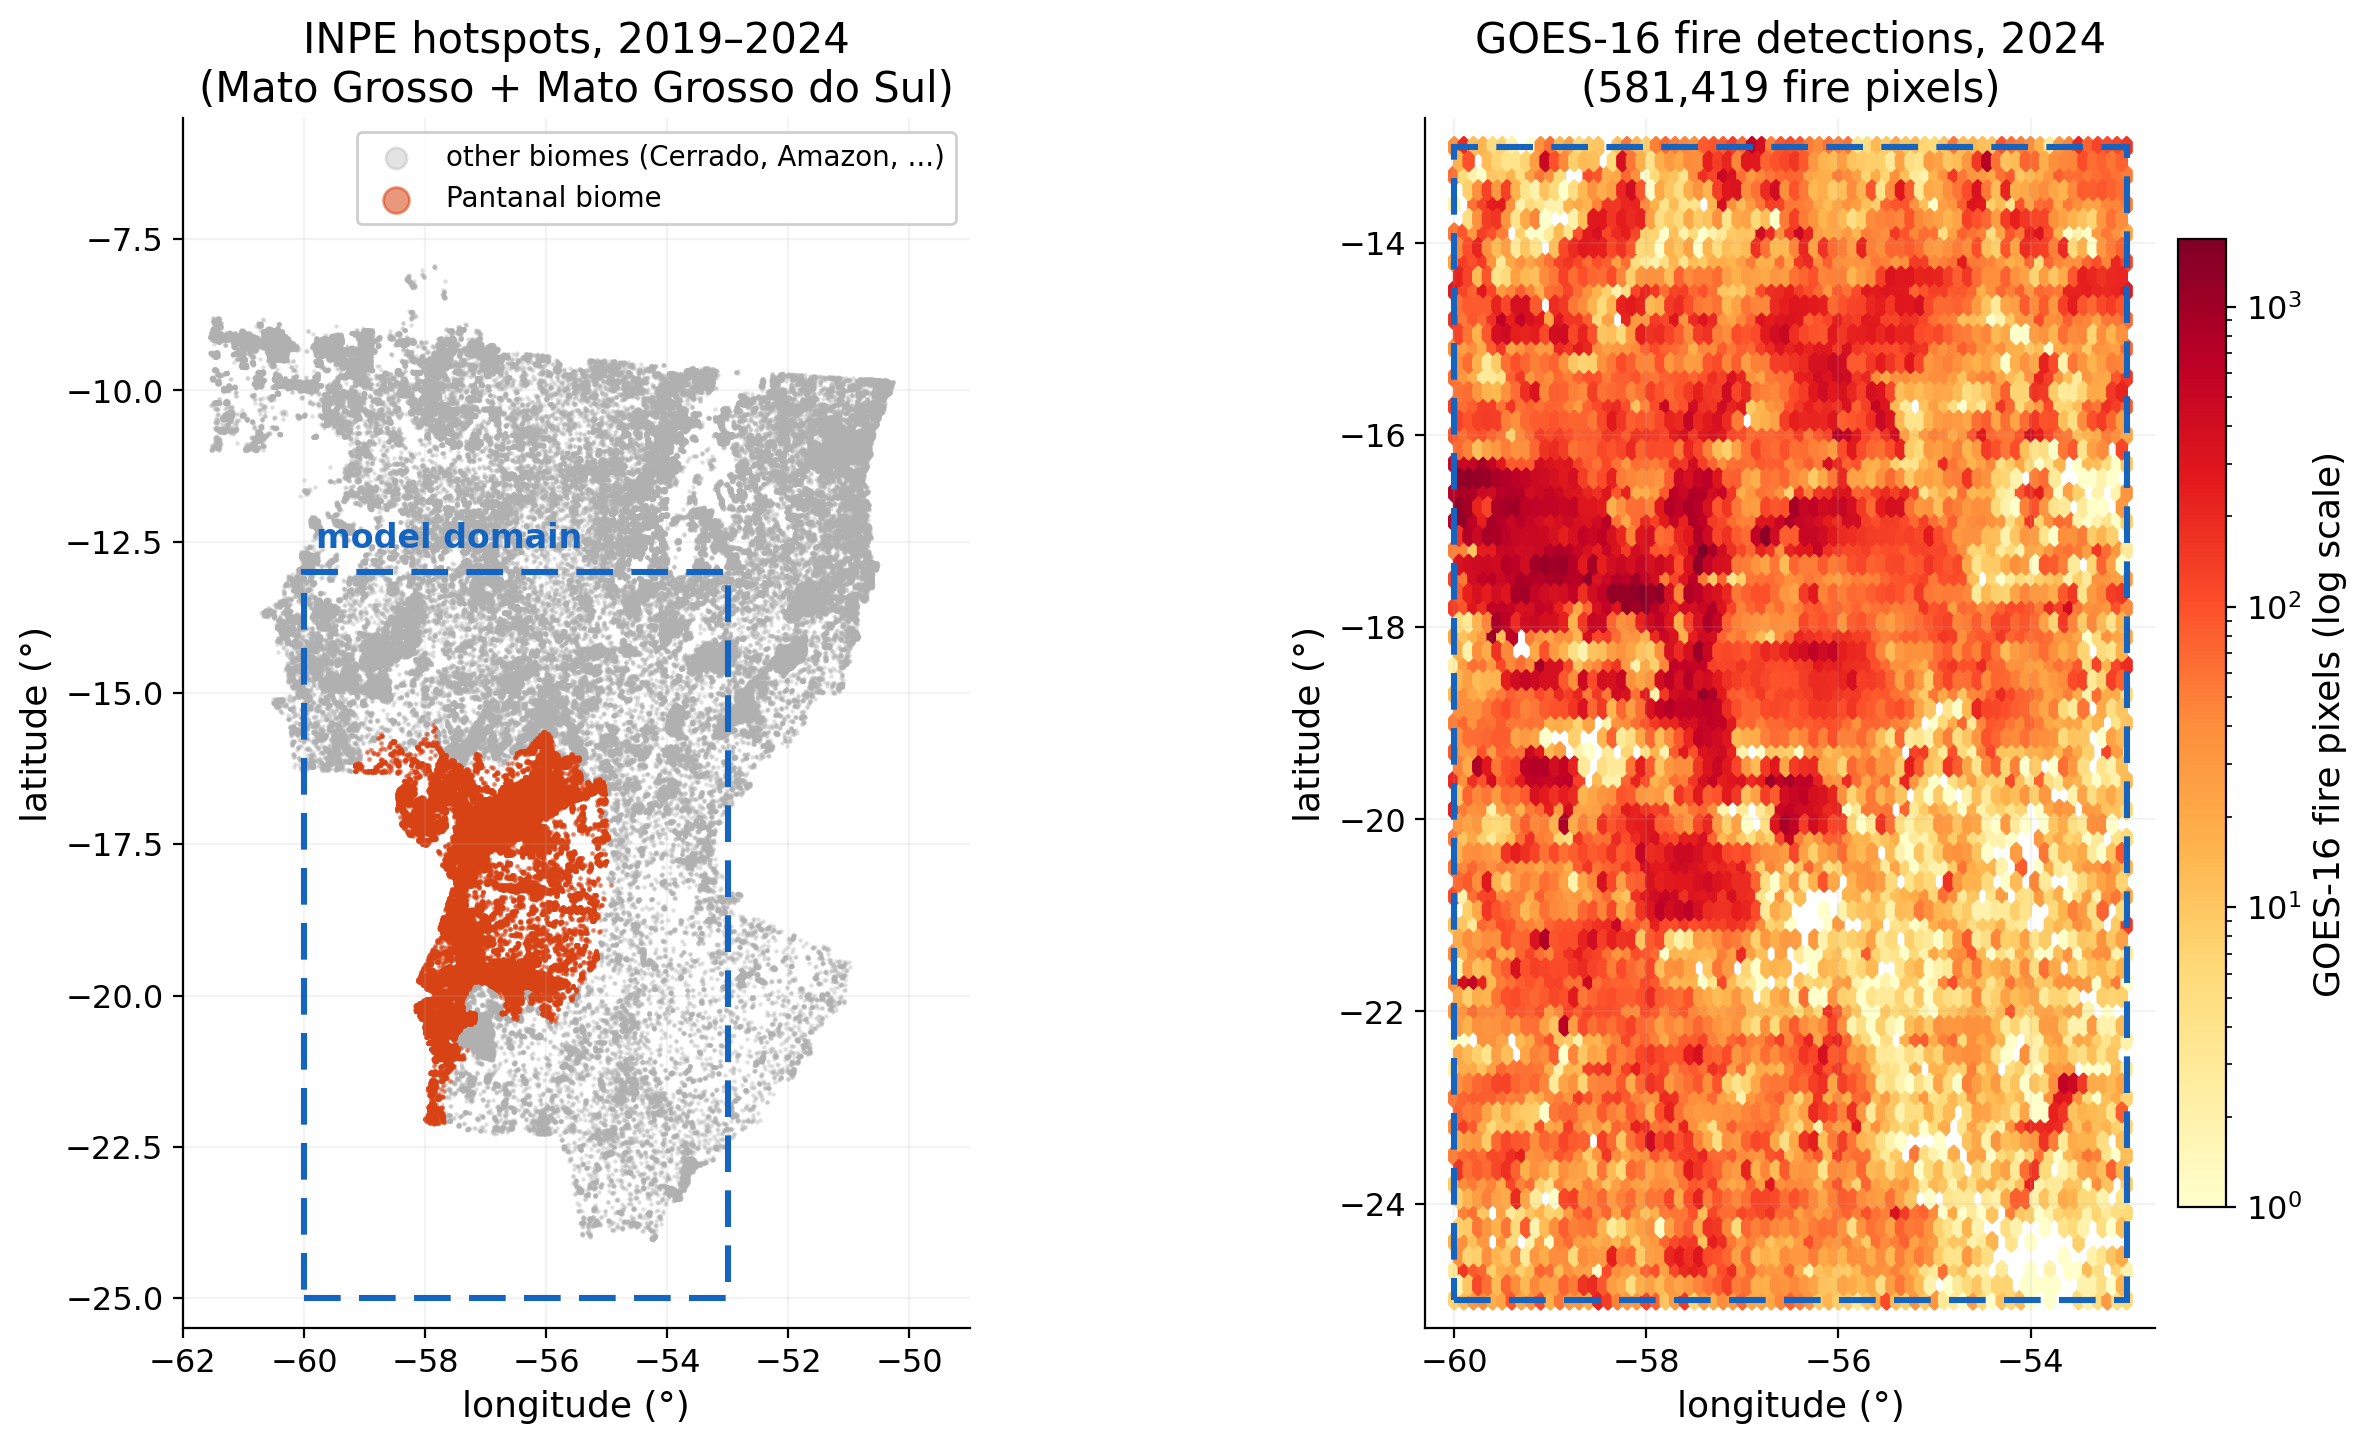
\includegraphics[width=\linewidth]{fig_study_area.png}
  \caption[Study area and fire detections]{Study area. \textbf{Left:} INPE
  reference-satellite fire detections, 2019--2024, in Mato Grosso and Mato Grosso
  do Sul; orange points fall in the Pantanal biome, grey points in other biomes.
  \textbf{Right:} density of GOES-16 fire pixels in 2024 inside the model domain
  (log colour scale). The dashed blue rectangle is the model domain
  ($13$--$25^\circ$S, $53$--$60^\circ$W).}
  \label{fig:study-area}
\end{figure}

All models share one rectangular domain, from $25^\circ$S to $13^\circ$S and
from $60^\circ$W to $53^\circ$W, which contains the whole Brazilian Pantanal. On
the ERA5 grid it is $49\times29$ cells of $0.25^\circ$.

\begin{warnbox}[Important: two slightly different study areas]
The two families of models do not cover exactly the same ground, and this
matters when comparing them.
\begin{itemize}
  \item The \textbf{INPE-based models} (Chapter~\ref{ch:inpe}) use only fire
        detections that INPE labels as \emph{Pantanal biome}, inside Brazil.
  \item The \textbf{GOES-16 models} (Chapters~\ref{ch:goes}--\ref{ch:spread}) use
        \emph{every} fire inside the rectangle: the Pantanal, but also
        surrounding Cerrado savanna and parts of Bolivia and Paraguay. As the
        right panel of Figure~\ref{fig:study-area} shows, the densest burning in
        2024 was actually on the western edge, towards Bolivia.
\end{itemize}
The GOES results should therefore be read as \enquote{the Pantanal and its
surroundings}. Restricting them to the biome only is straightforward with a
biome mask and is listed as future work.
\end{warnbox}

\section{Datasets}

Table~\ref{tab:datasets} lists every dataset used.

\begin{table}[H]
\centering\small
\caption{Datasets used in the project.}
\label{tab:datasets}
\begin{tabularx}{\linewidth}{>{\raggedright\arraybackslash}p{3.3cm} >{\raggedright\arraybackslash}X >{\raggedright\arraybackslash}p{2.4cm} >{\raggedright\arraybackslash}p{2.2cm}}
\toprule
\textbf{Dataset} & \textbf{What it is} & \textbf{Resolution} & \textbf{Period used} \\
\midrule
INPE Programa Queimadas, reference satellite (\code{Brasil\_sat\_ref}) &
Fire detections from Brazil's National Institute for Space Research. The
\enquote{reference satellite} series uses a single afternoon polar orbiter so
that counts are comparable across years. &
$\sim$1\,km; one overpass per day (16--19\,UTC) & 2019--2024 \\
\addlinespace
GOES-16 ABI L2 Fire/Hot Spot Characterization, Full Disk (\code{ABI-L2-FDCF}) &
Fire mask, fire radiative power (FRP), fire area and temperature from NOAA's
geostationary satellite, downloaded from NOAA's public cloud archive. &
$\sim$2\,km; every 10 min (1 scan/hour used) & 2024 \\
\addlinespace
ERA5 hourly data on single levels &
Reanalysis from ECMWF / Copernicus Climate Change Service: 2\,m temperature,
2\,m dew point, 10\,m wind components. RH and VPD derived from them. &
$0.25^\circ$ ($\sim$28\,km); hourly & 2019--2024 \\
\addlinespace
XHWI -- Extreme Heatwave Index & Hourly heatwave index produced by LAMMOC/UFF
(RiskClima project). & $0.25^\circ$; hourly & 2024 only \\
\addlinespace
Atmospheric blocking series & Daily counts of blocking events (total, north,
south, with lags), from the laboratory. & daily & 2019--2024 \\
\addlinespace
SACZ series & Daily indicators of the South Atlantic Convergence Zone, a major
rainfall system, from the laboratory. & daily & 2019--2024 \\
\addlinespace
SPI (\code{spiacc30}) & 30-day Standardized Precipitation Index. \emph{Not used}:
the series stops on 2024-10-19 and does not cover the full period. & daily & -- \\
\bottomrule
\end{tabularx}
\end{table}

\section{Software}

All code was written in Python: \code{pandas} and \code{numpy} for tables,
\code{xarray} and \code{h5py} for gridded satellite and weather files,
\code{scikit-learn} for the random forest, clustering and evaluation,
\code{xgboost} for gradient boosting, \code{optuna} for tuning,
\code{scipy} for statistics, \code{matplotlib} for figures, \code{cdsapi} to
download ERA5 and \code{boto3} to read the GOES-16 archive. Training ran on an
ordinary laptop: the largest table (600{,}000 rows) trains in minutes.

% =====================================================================
\chapter{Overall approach}\label{ch:method}
% =====================================================================

\section{Four stages}

The project did not follow a fixed plan decided on day one. Each stage answered a
question and exposed the limitation that motivated the next one
(Figure~\ref{fig:pipeline}).

\begin{figure}[H]
\centering
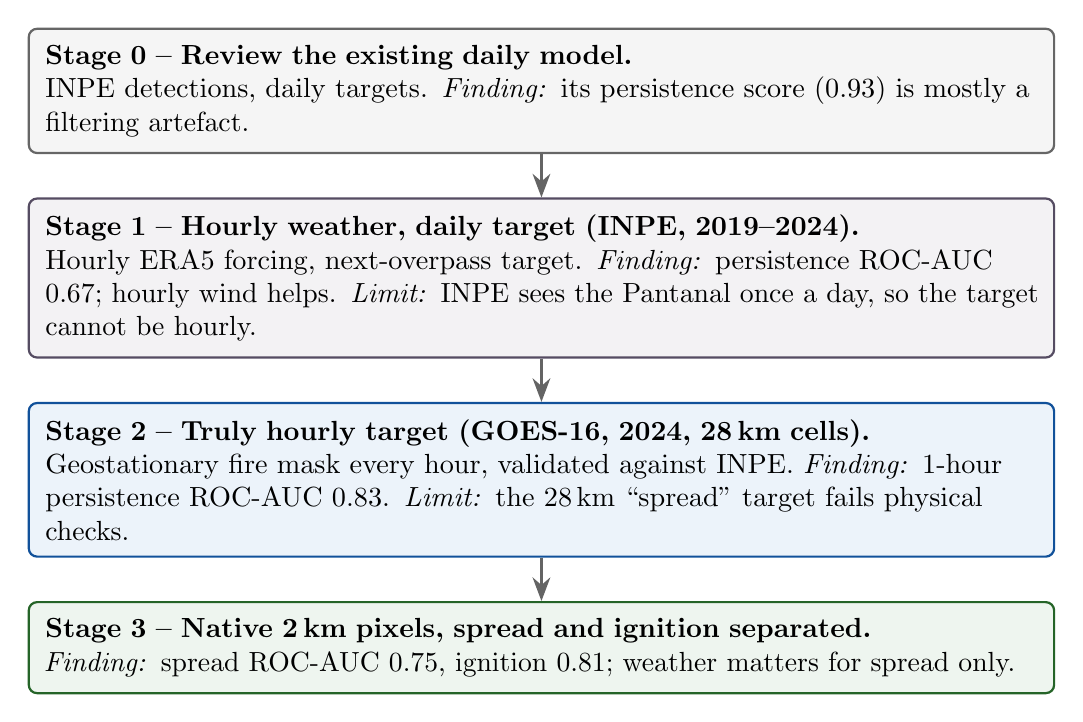
\begin{tikzpicture}[
  node distance=0.55cm,
  stage/.style={rectangle, rounded corners=3pt, draw=#1!80!black, fill=#1!8,
                line width=0.8pt, text width=12.6cm, inner sep=6pt, align=left},
  arr/.style={-{Stealth[length=3mm]}, line width=1pt, draw=ink!70}]
\node[stage=gray] (s0) {\textbf{Stage 0 -- Review the existing daily model.}\\
  INPE detections, daily targets. \emph{Finding:} its persistence score (0.93)
  is mostly a filtering artefact.};
\node[stage=inpe, below=of s0] (s1) {\textbf{Stage 1 -- Hourly weather, daily target (INPE, 2019--2024).}\\
  Hourly ERA5 forcing, next-overpass target. \emph{Finding:} persistence
  ROC-AUC 0.67; hourly wind helps. \emph{Limit:} INPE sees the Pantanal once a
  day, so the target cannot be hourly.};
\node[stage=goes, below=of s1] (s2) {\textbf{Stage 2 -- Truly hourly target (GOES-16, 2024, 28\,km cells).}\\
  Geostationary fire mask every hour, validated against INPE. \emph{Finding:}
  1-hour persistence ROC-AUC 0.83. \emph{Limit:} the 28\,km \enquote{spread}
  target fails physical checks.};
\node[stage=good, below=of s2] (s3) {\textbf{Stage 3 -- Native 2\,km pixels, spread and ignition separated.}\\
  \emph{Finding:} spread ROC-AUC 0.75, ignition 0.81; weather matters for
  spread only.};
\draw[arr] (s0) -- (s1);
\draw[arr] (s1) -- (s2);
\draw[arr] (s2) -- (s3);
\end{tikzpicture}
\caption[Project stages]{The four stages of the project. Each stage's limitation
motivated the next.}
\label{fig:pipeline}
\end{figure}

\section{Principles applied throughout}

\begin{description}
  \item[Time-ordered evaluation.] The test period always comes after the training
        period. Shuffling rows randomly would let the model see the same fire on
        both sides and inflate the scores.
  \item[Embargo.] Consecutive hours of the same fire are almost identical. A gap
        of 24\,h is left between training and test data so that the last training
        hour and the first test hour are not the same fire. Fire
        \enquote{chains} crossing the cut are removed from training.
  \item[Rolling origin.] Besides one large train/test split, models are also
        evaluated on several successive months (train up to month $m$, test month
        $m+1$). This shows whether results hold across the season rather than
        in one lucky period.
  \item[Fixed-hyperparameter comparisons.] To decide whether a group of features
        helps, all feature sets are trained with the \emph{same} fixed settings
        (400 trees, depth 5, learning rate 0.05) and several seeds, so that
        differences come from the features and not from tuning luck.
  \item[Absence of evidence is not evidence of absence.] A fire that is not
        detected is not necessarily extinguished; the satellite may simply not
        have looked. Rows whose outcome was not observed are removed, never
        labelled \enquote{no fire}.
\end{description}

% =====================================================================
\chapter{Stages 0--1: the INPE-based models}\label{ch:inpe}
% =====================================================================

\section{What \enquote{hourly} can mean with INPE data}

The INPE detections carry an exact time stamp, so at first sight they look
hourly. They are not. Over the Pantanal, the reference satellite passes only
between 16 and 19\,UTC, mostly at 17 and 18\,UTC (early afternoon local time), and in 2020--2024
\textbf{1{,}172 of the 1{,}189 Pantanal fire days (98.6\%) have detections in a
single hour} (Figure~\ref{fig:window}, left). The time stamp is hourly; the
\emph{sampling} is daily.

\begin{figure}[H]
  \centering
  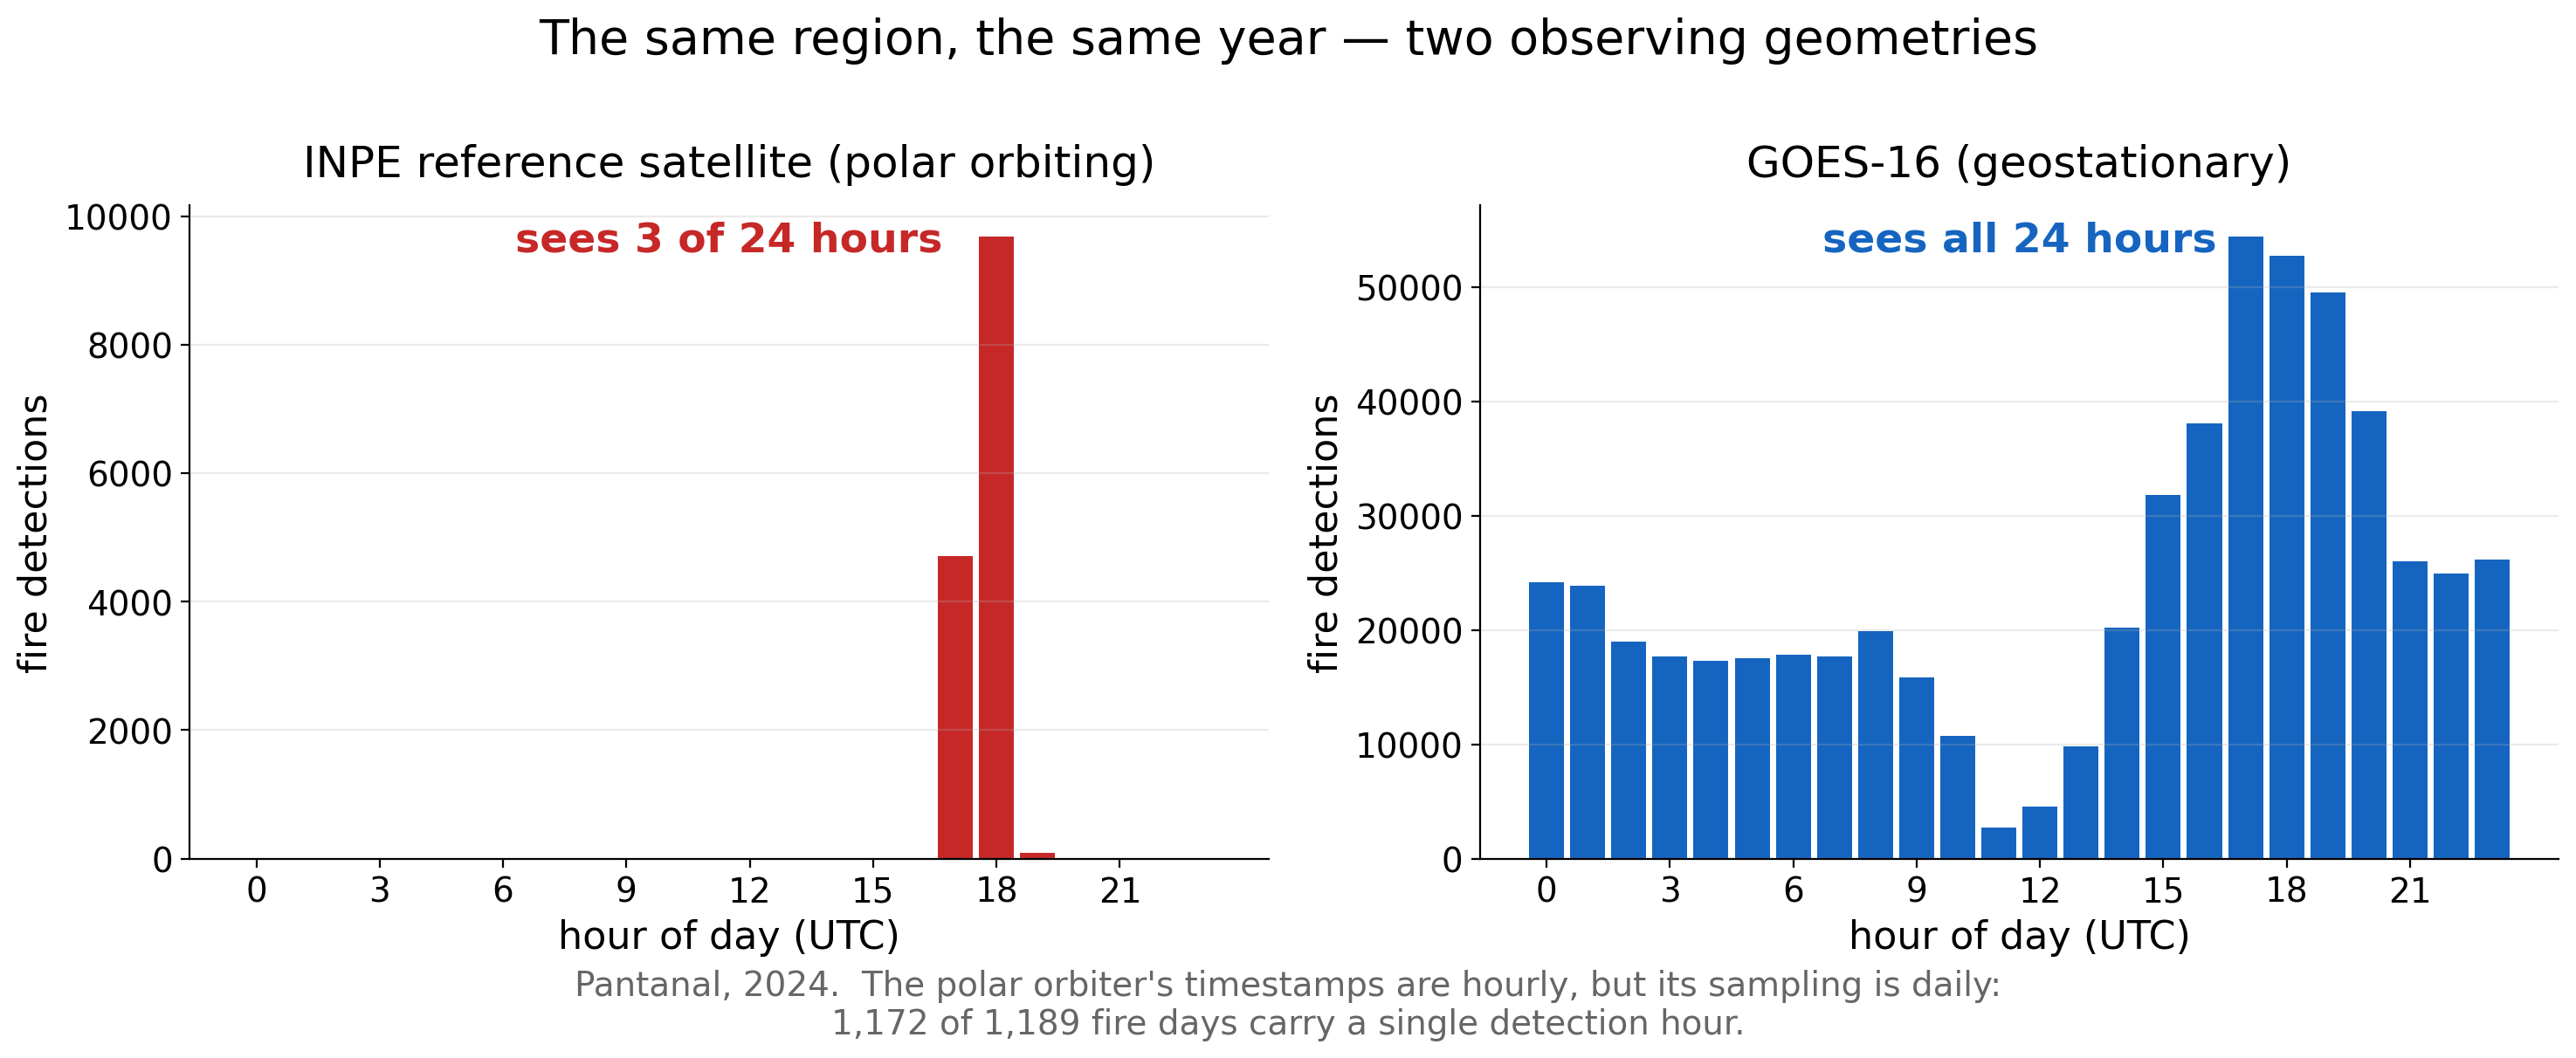
\includegraphics[width=\linewidth]{fig1_observing_window.png}
  \caption[Observing windows of INPE and GOES-16]{Fire detections by hour of day
  (UTC) in 2024. The polar orbiter used by INPE observes the Pantanal in only a
  few afternoon hours; GOES-16 observes all 24.}
  \label{fig:window}
\end{figure}

Consequently the Stage-1 model has an \textbf{hourly forcing} but a
\textbf{daily target}: it predicts what happens at the next overpass (about
24\,h later), but describes the weather hour by hour at the time of detection
and over the preceding 24\,h, instead of using daily averages.

\section{From detections to fire events}

\paragraph{Grouping detections into clusters.} Nearby detections from the same
overpass usually belong to the same fire. They were grouped with
\textbf{DBSCAN}, a clustering method that links points closer than a chosen
distance. A distance of 1.4\,km reproduced the laboratory's original grouping
almost exactly (agreement score ARI = 0.974, where 1 is identical), and the same
rule was then applied to every year so that the six years are consistent.

\paragraph{Linking clusters over time.} A cluster is linked to one seen at the
next overpass if they are within \textbf{5\,km}; linked clusters form a
multi-day \emph{chain}, i.e.\ one fire followed through time.

\paragraph{Targets.}
\begin{itemize}
  \item \code{persists\_t1} = 1 if some cluster is detected within 5\,km at the
        next overpass;
  \item \code{spreads\_t1} = 1 if a \emph{new} cluster (one that starts its own
        chain) appears in the ring between 5 and 20\,km.
\end{itemize}

\paragraph{Was the next day observed?} If nothing is detected the next day, it
could mean the fire went out -- or that the satellite did not pass. To tell the
two apart, detections anywhere in Mato Grosso and Mato Grosso do Sul were used as
proof that the satellite did observe the region that day. Clusters whose next
day was not observed were \emph{removed}, not labelled \enquote{extinguished}.

\begin{warnbox}
Restricting the input to Pantanal-biome detections \emph{before} this test
removed exactly the evidence that the satellite had passed: 433 clusters were
wrongly dropped as \enquote{next day unobserved}, instead of 76. The data are now
scoped by state (MS + MT) and the biome filter is applied afterwards.
\end{warnbox}

\section{Data volume}

From 2019 to 2024 there were \textbf{63{,}114} Pantanal detections, forming
27{,}443 clusters, of which \textbf{26{,}951} were kept (492 had an unobserved
next day). Table~\ref{tab:inpe-years} shows how uneven the years are: 2020 was
catastrophic, 2022 very quiet.

\begin{table}[H]
\centering\small
\caption{INPE-based dataset by year (Pantanal biome).}
\label{tab:inpe-years}
\begin{tabular}{lrrr}
\toprule
Year & Fire clusters & Share persisting next day & Share spreading \\
\midrule
2019 & 4{,}695 & 0.300 & 0.257 \\
2020 & \textbf{9{,}851} & \textbf{0.429} & \textbf{0.324} \\
2021 & 3{,}563 & 0.335 & 0.224 \\
2022 & 845 & 0.230 & 0.082 \\
2023 & 2{,}427 & 0.343 & 0.255 \\
2024 & 5{,}570 & 0.422 & 0.286 \\
\bottomrule
\end{tabular}
\end{table}

\begin{figure}[H]
  \centering
  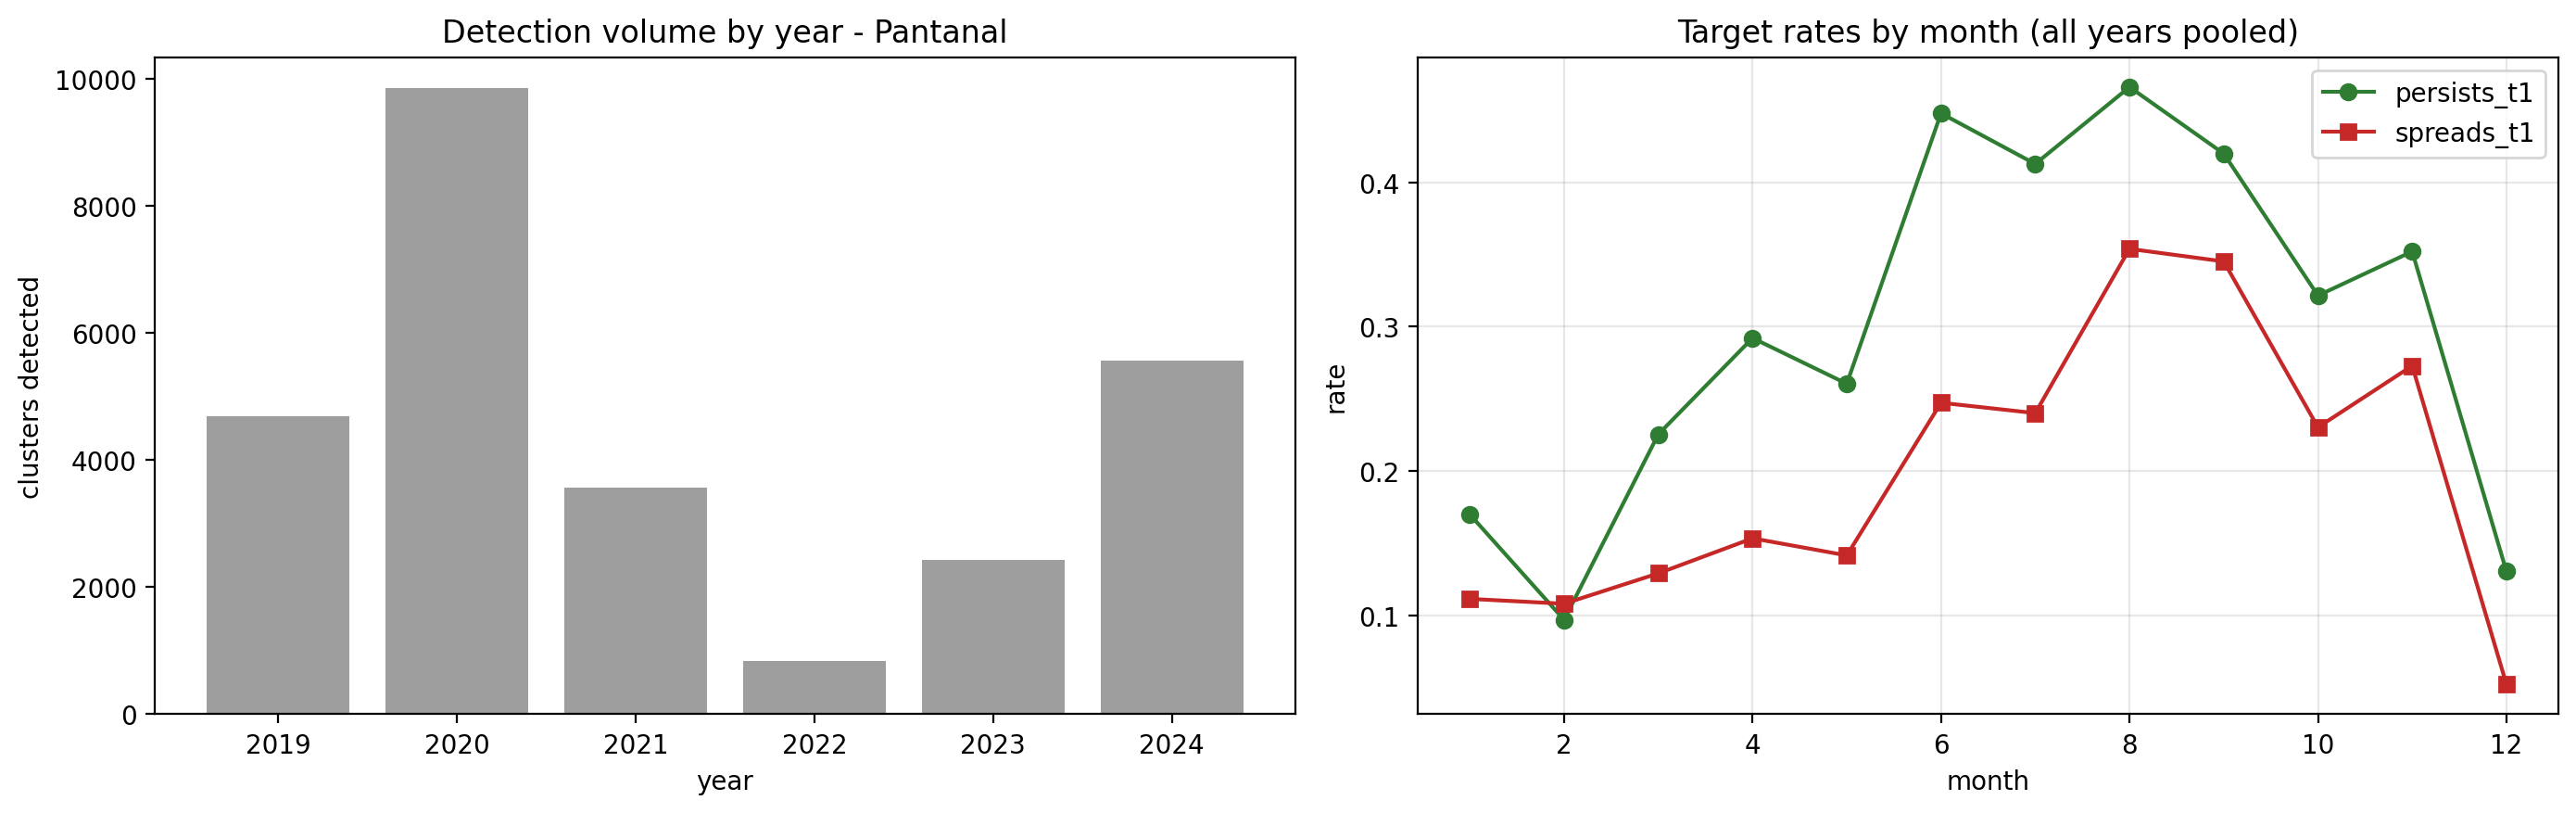
\includegraphics[width=\linewidth]{fig_inpe_overview.png}
  \caption[INPE dataset overview]{INPE-based dataset. \textbf{Left:} number of
  fire clusters per year. \textbf{Right:} share of clusters that persist or
  spread, by calendar month (all years pooled): both peak in the dry season
  (June--September).}
  \label{fig:inpe-overview}
\end{figure}

\section{Features}

Features were organised in blocks so that the contribution of each block could be
tested (the full list is in Appendix~\ref{app:features}):

\begin{description}
  \item[Baseline (27 features)] -- what the daily model could see: position, number
        of detections, how many days the fire has already lasted, season, year,
        \emph{daily} ERA5 averages and maxima, atmospheric blocking and SACZ.
  \item[Hourly block (37)] -- hourly temperature, humidity and VPD at the time of
        detection and 1--12\,h before, their 24\,h minimum/maximum/mean, the
        number of hours above 32\,$^\circ$C or below 30\% humidity; plus the
        \emph{geometry} of the cluster (size, elongation, distance to the nearest
        other fire, number of fires in the ring, movement since the last
        overpass).
  \item[Hourly wind (13)] -- hourly wind speed, components and direction, their
        variability, and the alignment between wind and the fire's movement.
\end{description}

\paragraph{Why not use the XHWI heatwave index?} XHWI exists only for 2024. Using
it would have meant throwing away five of the six years. Instead, the raw
quantities XHWI is built from (temperature, humidity, VPD) were used directly
for all years, together with a count of hours above 32\,$^\circ$C that mimics
XHWI's temperature threshold. The code automatically adds the XHWI block if it
ever becomes available for every year. As it turned out, humidity was the most
informative weather variable, which a temperature-based index would have partly
hidden.

\section{Train and test split}

The model was trained on \textbf{2019--2022} (18{,}954 clusters) and tested on
\textbf{2023--2024} (7{,}997 clusters). The training period contains both an
extreme year (2020) and a quiet one (2022); the test period contains one weak and
one strong year. In the test set the base rates are 0.398 (persistence) and
0.276 (spread).

\section{Results}

\begin{table}[H]
\centering\small
\caption[INPE-based model scores]{INPE-based model, test 2023--2024, tuned models.
Persistence is scored by ROC-AUC (chance = 0.5), spread by PR-AUC (chance =
0.276).}
\label{tab:inpe-results}
\begin{tabular}{llccc}
\toprule
Target & Model & Baseline & + hourly & + hourly + wind \\
\midrule
\multirow{2}{*}{Persistence (ROC-AUC)} & XGBoost & 0.632 & 0.659 & \textbf{0.670} \\
 & Random forest & 0.606 & 0.656 & 0.656 \\
\midrule
\multirow{2}{*}{Spread (PR-AUC)} & XGBoost & 0.367 & 0.385 & \textbf{0.389} \\
 & Random forest & 0.325 & 0.345 & 0.364 \\
\bottomrule
\end{tabular}
\end{table}

The best spread model has ROC-AUC 0.652 and a lift of 1.41 (its alarms are 41\%
more often correct than random).

\subsection{Reproducibility and the noise floor}

\begin{warnbox}[Pitfall: the same run gave two different answers]
Re-running an \emph{identical} configuration moved persistence ROC-AUC from 0.631
to 0.601 -- as large as the differences between feature sets. The cause: the
estimator was seeded, but Optuna's search was not, so each run tried different
hyperparameters. Every tuning study is now seeded and runs reproduce exactly.
The laboratory's daily notebook has the same issue, so its small differences
carry the same caveat.
\end{warnbox}

Seeding makes a result reproducible, not significant. The feature blocks were
therefore compared with fixed hyperparameters over five seeds
(Table~\ref{tab:inpe-effect}).

\begin{table}[H]
\centering\small
\caption[INPE effect-size test]{Effect-size test with fixed hyperparameters, 5
seeds (test 2023--2024). \sig{} = seed-to-seed noise.}
\label{tab:inpe-effect}
\begin{tabular}{lcccc}
\toprule
 & \multicolumn{2}{c}{Persistence (ROC-AUC)} & \multicolumn{2}{c}{Spread (PR-AUC)} \\
\cmidrule(lr){2-3}\cmidrule(lr){4-5}
Feature set & mean & vs baseline & mean & vs baseline \\
\midrule
Baseline & 0.6208 & -- & 0.3554 & -- \\
+ hourly & 0.6333 & +0.0125 (1.6\sig) & 0.3443 & $-$0.0111 ($-$1.0\sig) \\
+ hourly + wind & \textbf{0.6472} & \textbf{+0.0265 (3.4\sig)} & 0.3615 & +0.0061 (0.5\sig) \\
+ hourly + wind + timing & 0.6436 & +0.0228 (2.9\sig) & 0.3358 & $-$0.0197 ($-$1.7\sig) \\
\bottomrule
\end{tabular}
\end{table}

\begin{keybox}
For next-day persistence, hourly weather gives a real gain (+0.027 ROC-AUC,
3.4\sig), mostly thanks to \textbf{hourly wind}. For next-day spread, no block of
features gives an effect distinguishable from noise.
\end{keybox}

\paragraph{Where the skill comes from.} Removing whole blocks at fixed settings
showed that the \textbf{geometry} of the fire (how large it is, how close it is
to other fires, how many fires surround it) is the strongest block: persistence
fell from 0.636 to 0.600 without it. The atmosphere alone still gave 0.609, with
\textbf{relative humidity} the most informative weather variable.

\paragraph{Data volume mattered most.} A first version built on 2024 alone scored
at chance (ROC-AUC 0.479--0.526). Six years of data are what made the model work
at all: a single year contains no information about the year-to-year differences
in fire severity.

\subsection{Timing features: important but harmful}\label{sec:timing}

Two features describing the timing of the overpass (the hour of detection and the
time until the next overpass) ranked near the top of XGBoost's importance.
Removing them \emph{improved} persistence from 0.636 to 0.648 and left spread
unchanged; adding them back to the final set also made both targets worse
(Table~\ref{tab:inpe-effect}, last row). They were dropped. This is the clearest
illustration of the rule \enquote{importance is not usefulness}.

\begin{warnbox}[Leak: the time to the next overpass]
The time until the next overpass was first computed from Pantanal detections. On
days with no fire it was undefined and filled with 24\,h -- so the value itself
revealed that the fire had not persisted (persistence rate 0.218 at the filled
value against 0.477 elsewhere). It was recomputed from regional overpass times,
which exist whatever burns, and then removed from the features anyway.
\end{warnbox}

\section{Comparison with the daily model}\label{sec:daily-artifact}

The laboratory's daily model reports a persistence ROC-AUC of about
\textbf{0.93}, far above the 0.67 obtained here. Looking into the reason
revealed that the two numbers do not measure the same thing.

The daily table contains only fires that lasted \emph{at least two days}: of
7{,}311 Pantanal events, only 34 have a single row. So on the first day of any
event, a second day exists \emph{by construction}. In the daily test set,
\enquote{the fire has lasted 0 days so far} implies \enquote{it persists} in
1{,}204 out of 1{,}204 rows. The one-line rule
\begin{center}
\code{persists = (days\_already\_burning == 0)}
\end{center}
with no model at all scores \textbf{accuracy 0.896, F1 0.896, ROC-AUC 0.905}. The
tuned XGBoost scores F1 0.895 -- no better -- and ROC-AUC 0.932, only +0.03
above the trivial rule.

\begin{table}[H]
\centering\small
\caption{Daily versus hourly model (INPE, test 2023--2024).}
\label{tab:daily-vs-hourly}
\begin{tabular}{lcc}
\toprule
 & Daily model & Hourly-forcing model \\
\midrule
Question actually answered & \makecell{``given this fire lasts $\geq$2 days,\\ is today day one?''} & \makecell{``will this fire still\\ be here tomorrow?''} \\
Trivial-rule F1 & 0.896 & 0.400 \\
Model F1 & 0.895 & 0.604 \\
Gain over trivial rule & $\approx 0$ & +0.204 \\
\midrule
Spread: base rate & 0.292 & 0.276 \\
Spread: best PR-AUC (lift) & 0.469 (1.61$\times$) & 0.389 (1.41$\times$) \\
\bottomrule
\end{tabular}
\end{table}

\begin{keybox}[Key result: the daily persistence score is an artefact]
The daily model's 0.93 should not be quoted as predictive skill; it mostly
reflects how its table was filtered. The hourly model scores lower on a harder,
unfiltered and more useful question -- in practice one does not know in advance
which fires will last two days. For \textbf{spread}, where no such artefact
exists, the daily model is genuinely somewhat ahead (lift 1.61 vs 1.41), though
on a smaller and more selected test set.
\end{keybox}

Two other observations about the daily model: its wind features changed scores
by at most $\pm$0.013, well within tuning noise; and the wind direction it uses
appears to follow the meteorological convention (the direction the wind comes
\emph{from}), which would invert the meaning of its wind--fire alignment feature.
The new pipeline stores only the direction the wind blows \emph{to}, to avoid
this confusion.

% =====================================================================
\chapter{Stage 2: a truly hourly target with GOES-16}\label{ch:goes}
% =====================================================================

\section{Why the INPE product cannot give an hourly target}

One could try to build an hourly target from INPE by treating every hour without
a detection as \enquote{no fire}. This \emph{zero-fill} approach fails badly: the
base rate becomes 0.000886 (less than 0.1\%), and \textbf{the hour of the day
alone predicts \enquote{fire} with ROC-AUC 0.917} -- simply because detections
only exist in the hours the satellite passes. Such a model would learn the
satellite's orbit, not fire behaviour. A satellite that actually looks every hour
was needed.

\section{The GOES-16 fire product}\label{sec:goes-product}

GOES-16 is NOAA's geostationary satellite covering the Americas. Its fire product
gives, for each $\sim$2\,km pixel, a \textbf{mask code} that distinguishes three
situations (Table~\ref{tab:mask}). This three-way distinction is what makes an
hourly target possible: a zero now means \enquote{observed, no fire}.

\begin{table}[H]
\centering\small
\caption{How GOES-16 mask codes were used.}
\label{tab:mask}
\begin{tabular}{lll}
\toprule
Mask codes & Meaning & Used as \\
\midrule
10--15, 30--35 & fire detected (various confidence levels) & fire (1) \\
100 & observed, no fire & no fire (0) \\
40, 50, 60, 120 and above & cloud, water, bad data, not processed & not observed (excluded) \\
\bottomrule
\end{tabular}
\end{table}

For each $0.25^\circ$ ERA5 cell and each hour, the fraction of its pixels that
were actually observed (\code{obs\_frac}) was computed; cell-hours with less than
half the pixels observed were excluded.

\paragraph{Locating the pixels.} GOES-16 images are in a special
\enquote{fixed-grid} projection (angles seen from the satellite). A small module
was written to convert these to latitude and longitude, tested to a round-trip
error of $10^{-14}$ degrees. The Pantanal window is 615\,$\times$\,420 pixels --
0.88\% of the full disk -- containing 211{,}324 land pixels that map onto 1{,}421
ERA5 cells (about 149 pixels per cell).

\begin{warnbox}[Engineering: 40 times faster]
Each GOES file covers the whole disk from Alaska to Patagonia. Decoding it with
the standard library took 3.3\,s per file. Reading only the Pantanal window
directly from the HDF5 file took 83\,ms, with identical output. At 8{,}784 files
per year this is the difference between 8 hours and 12 minutes of processing.
\end{warnbox}

\section{Validation against INPE: August 2024}

Before trusting GOES-16, one month (August 2024, 744 hours, all present) was
compared with INPE:

\begin{itemize}
  \item 919{,}743 observed cell-hours, of which 3.99\% contained fire;
  \item coverage was excellent: median \code{obs\_frac} = 1.000, and 90.8\% of
        cell-hours had at least 90\% of pixels observed;
  \item of the 517 cell-hours where INPE detected fire, GOES-16 also detected fire
        in \textbf{403 (77.9\%)}. INPE passes in the afternoon, when many cells
        burn: at those same hours a randomly chosen cell has GOES fire 10.1\% of
        the time, so the agreement is \textbf{about 8 times better than chance}.
        (Comparing with the fire rate averaged over all hours of the month, 3.8\%,
        would give 20 times, but that baseline is too easy.) Perfect agreement is
        not expected, since the two instruments have different resolution and
        sensitivity.
\end{itemize}

\begin{figure}[H]
  \centering
  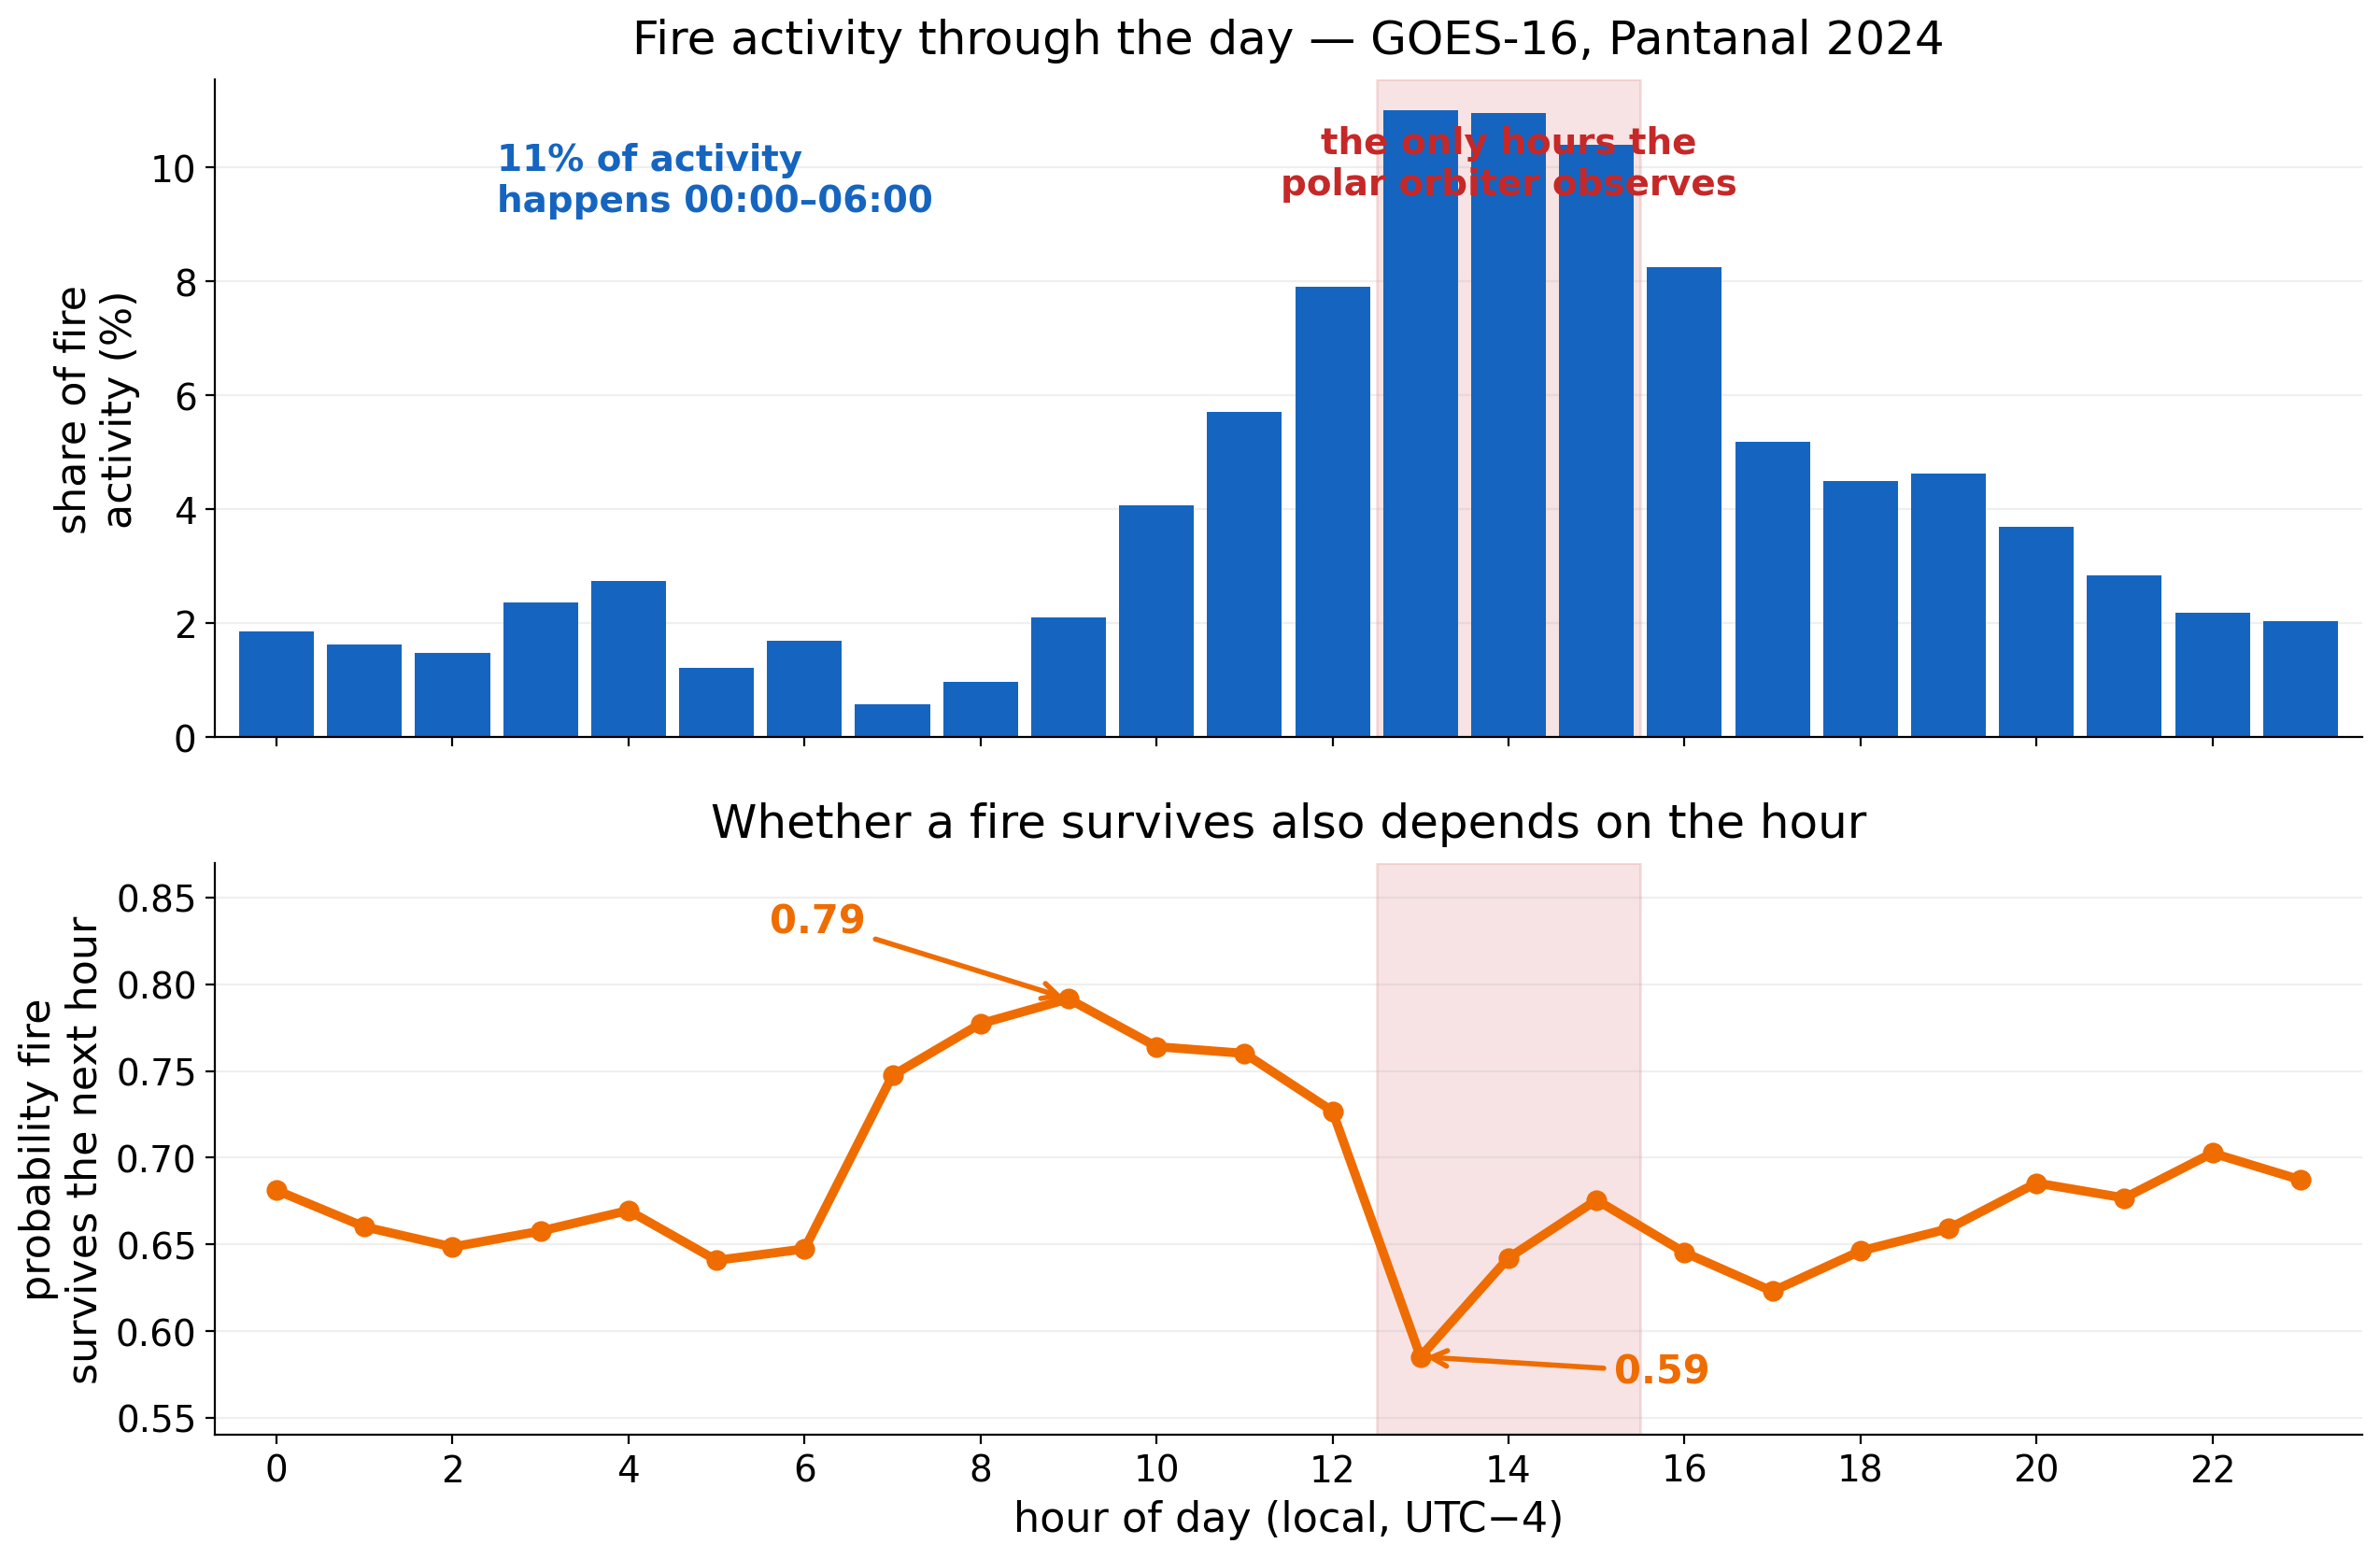
\includegraphics[width=0.92\linewidth]{fig2_diurnal_cycle.png}
  \caption[The fire diurnal cycle seen by GOES-16]{What GOES-16 reveals.
  \textbf{Top:} share of fire activity by local hour (2024); the red band marks
  the only hours the polar orbiter observes. \textbf{Bottom:} probability that a
  burning cell is still burning one hour later, by local hour.}
  \label{fig:diurnal}
\end{figure}

GOES-16 shows a strong \textbf{daily cycle} that INPE cannot see
(Figure~\ref{fig:diurnal}). In August, fire activity peaks at 14:00 local time
(9.0\% of cell-hours burning) and is lowest at 06:00 (1.16\%) -- a factor of 7.8.
About 10--11\% of all fire activity occurs between midnight and 06:00, entirely
invisible to an afternoon polar orbiter. Over the whole year, the probability
that a fire survives the next hour is highest at 09:00 (0.79) and lowest at 13:00
(0.59), when many short-lived fires start and die.

\begin{plainbox}
With GOES-16, the hour of the day becomes a legitimate feature. With INPE it only
encoded when the satellite happened to pass; with GOES-16 it encodes the real
daily rhythm of fire, driven by the sun, temperature and humidity.
\end{plainbox}

\section{The hourly model on 28\,km cells}

\paragraph{Table.} All of 2024 was downloaded (one scan per hour). Fire was
aggregated onto the ERA5 grid and joined to the hourly weather. For every cell
burning at hour $t$ (130{,}550 rows), two targets were defined:
\begin{itemize}
  \item \code{persists\_t1h}: the same cell is still burning at $t+1$\,h (base
        rate 0.674);
  \item \code{spreads\_t1h}: a neighbouring cell that was not burning at $t$ is
        burning at $t+1$\,h (base rate 0.207).
\end{itemize}

\paragraph{Features.} Three blocks: \emph{context} (position, hour of day, day of
year), \emph{fire state} (number of fire pixels, fire area, fire radiative power,
fire history over the last 1--24\,h, fire in neighbouring cells), and
\emph{meteorology} (temperature, humidity, VPD and wind now, 1--12\,h before and
over 24\,h).

\paragraph{Strong seasonality.} Persistence ranges from \textbf{0.446 in
February} to \textbf{0.753 in September}: a fire in the wet season has roughly
even odds of surviving the hour, one in September three in four. A single test
period averages over this, which is why results were also checked month by month.
GOES-16 also sees wet-season fires far better than INPE: January--May holds 21\%
of the GOES rows against 6\% of INPE's annual detections.

\paragraph{Results.} Training on January--August (80{,}012 rows) and testing on
September--December (49{,}039 rows), with fixed hyperparameters and 5 seeds:

\begin{table}[H]
\centering\small
\caption[GOES-16 28\,km model, holdout]{GOES-16 hourly model on 28\,km cells, test
September--December 2024.}
\label{tab:goes-holdout}
\begin{tabular}{lcccc}
\toprule
 & \multicolumn{2}{c}{Persistence in 1\,h (ROC-AUC)} & \multicolumn{2}{c}{Spread in 1\,h (PR-AUC)} \\
\cmidrule(lr){2-3}\cmidrule(lr){4-5}
Feature set & score & gain & score & gain \\
\midrule
Context only & 0.6415 & -- & 0.3355 & -- \\
+ fire state & \textbf{0.8302} & +0.1887 (164\sig) & 0.3908 & +0.0553 (15\sig) \\
+ meteorology & 0.8308 & +0.0006 & 0.3926 & +0.0018 \\
\bottomrule
\end{tabular}
\end{table}

The tuned XGBoost reached ROC-AUC 0.830 for persistence and ROC-AUC 0.715 /
PR-AUC 0.394 for spread. On five monthly folds (June--October), the fire-state
block helped in 5 of 5 folds for both targets ($t=14.4$ and $t=11.5$).

\begin{keybox}
Knowing what the fire is doing \emph{now} lifts one-hour persistence from 0.64 to
0.83. Adding weather on top changes nothing: over one hour, the weather does not
change enough to alter a fire's fate.
\end{keybox}

\section{Feature decisions and bugs fixed}

\begin{warnbox}[Pitfall: \enquote{not measured} is not \enquote{zero}]
GOES-16 often detects a fire but cannot measure its power, area or temperature
(power is available for about 80\% of burning cell-hours). These gaps had been filled
with 0. The model then learned that \enquote{zero power} means \enquote{short-lived}
(persistence 0.55 versus 0.77), which was really a \emph{measurement-failure}
flag disguised as a physical value. Missing values are now left missing (the
algorithms handle this natively), and explicit flags record whether each
measurement exists.
\end{warnbox}

Other decisions: the day of the month was removed (an index, not a physical
quantity) and replaced by a smooth seasonal cycle; the observed fraction
\code{obs\_frac} is used only as a quality filter, not as a feature, so the model
cannot learn cloud patterns; a true fire area in km$^2$ was added, because GOES
pixels get larger away from the point under the satellite.

\begin{warnbox}[Two silent bugs]
\textbf{A missing month.} A network interruption during the download of April
2024 aborted that month without error; the year silently had eleven months.
Every download now retries with increasing delays and failures are reported
loudly.\\[0.3em]
\textbf{Shifted history.} The \enquote{fire 1 hour ago} feature was computed by
taking the previous \emph{row}. Where an hour was missing (a failed scan), it
reached back 2 hours instead. The time axis is now built from a complete list of
hours, so gaps stay gaps. About 1.6\% of hours were affected -- a bug that would
never have shown up in the scores.
\end{warnbox}

% =====================================================================
\chapter{Stage 3: getting spread right}\label{ch:spread}
% =====================================================================

\section{The 28\,km spread target was not measuring spread}

Three physical checks were applied to the spread target of Stage 2:

\begin{enumerate}
  \item \textbf{Speed.} Reaching the next 28\,km cell within one hour requires a
        fire front moving at about \textbf{7.7\,m/s} ($\approx$28\,km/h). Even the
        fastest crown fires rarely exceed 1--3\,m/s.
  \item \textbf{Direction.} If fire truly spreads, it should favour the
        downwind direction. Only 25.4\% of \enquote{spread} events were within
        $45^\circ$ of downwind -- exactly the 25\% expected at random.
  \item \textbf{Fire power.} More intense fires should spread more. Across five
        classes of fire radiative power, persistence rose steeply (0.45 to 0.97),
        but the spread rate rose much less (0.14 to 0.23) and levelled off in the
        top two classes. This check is weaker than the first two: the speed and
        direction checks are the decisive ones.
\end{enumerate}

The target was really measuring \enquote{some new fire appeared somewhere within
about 28\,km} -- mostly unrelated fires. The 28\,km cell had been chosen to match
the weather grid, but it discarded a factor of 14 in resolution in exactly the
dimension where spread happens (Figure~\ref{fig:resolution}).

\begin{figure}[H]
  \centering
  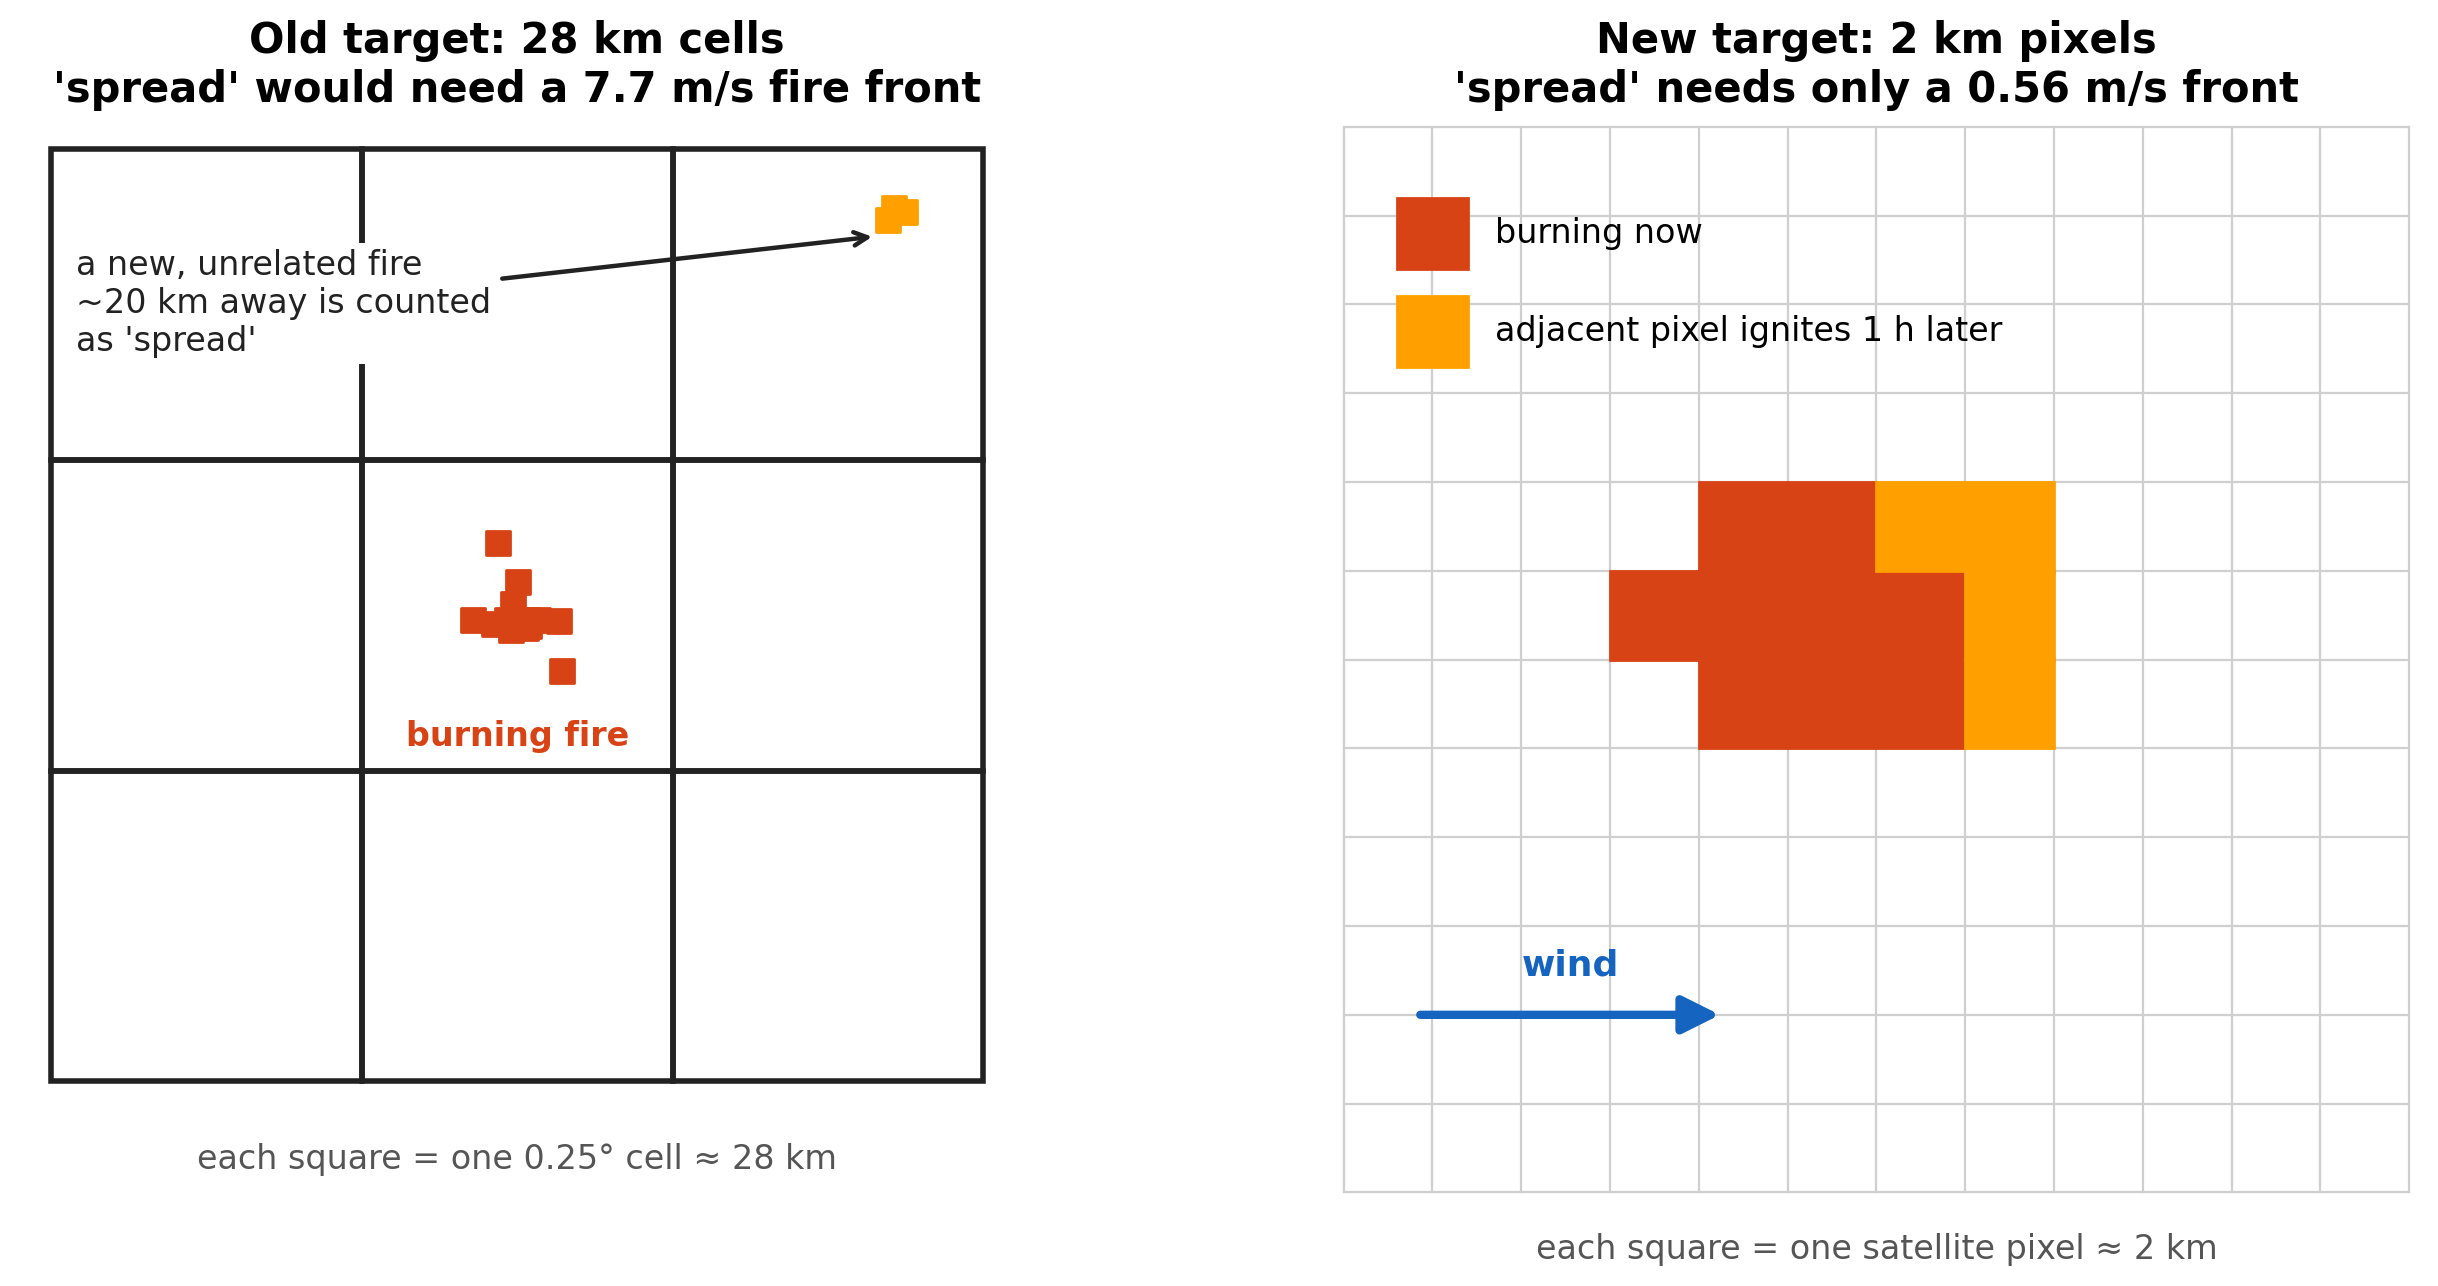
\includegraphics[width=\linewidth]{fig_resolution.png}
  \caption[Why the spread target needed 2\,km pixels]{Why resolution matters for
  spread. \textbf{Left:} on 28\,km cells, an unrelated fire appearing $\sim$20\,km
  away counts as \enquote{spread}. \textbf{Right:} on 2\,km pixels, spread means
  fire reaching adjacent ground, which is physically plausible within an hour.}
  \label{fig:resolution}
\end{figure}

\section{The fix: store fire at native resolution and split the target}

\paragraph{A native-pixel store.} Every GOES-16 fire pixel of 2024 was stored
with its exact position and properties: \textbf{581{,}419 fire pixels in only
9.1\,MB}, because fire pixels are sparse. Any new target definition now takes
minutes of computation instead of a full re-download.

\paragraph{Two separate questions.} The old target mixed two processes with
different causes. They were separated:

\begin{description}
  \item[Spread (2\,km).] For each burning pixel that has at least one unburnt
        neighbour: does an adjacent pixel that was not burning ignite in the next
        hour? (478{,}640 rows, base rate 0.194.) Pixels surrounded by fire on all
        eight sides are excluded -- they have nowhere to go.
  \item[Ignition.] For each weather cell with no fire in it or in the cells
        around it: does fire appear in the next hour? This is rare: 27{,}895
        ignitions out of 7{,}098{,}138 eligible cell-hours (0.39\%). To keep the
        table manageable, non-events were sampled at 20 per event (599{,}471 rows,
        artificial base rate 0.047). ROC-AUC is unaffected by this sampling;
        PR-AUC is only comparable between models on this same table.
\end{description}

\begin{warnbox}[Leakage guard]
Some columns describe \emph{where} the fire went (the bearing of the spread, whether
it went downwind). They are needed for the physical checks but are only known
after the fact. They are excluded from every feature set, and the code refuses to
run if one of them appears among the features.
\end{warnbox}

\section{The physical checks now pass}

\begin{table}[H]
\centering\small
\caption{Physical checks on the spread target, before and after the fix.}
\label{tab:checks}
\begin{tabular}{lcc}
\toprule
Check & Old target (28\,km) & New target (2\,km) \\
\midrule
Implied front speed & 7.7\,m/s (impossible) & \textbf{0.56\,m/s} (physical) \\
Spread within $45^\circ$ of downwind & 25.4\% (= random) & \textbf{28.6\%} ($z=25.6$) \\
Spread rate by fire power$^\ast$ & 0.14 $\rightarrow$ 0.23, levels off & \textbf{0.109 $\rightarrow$ 0.273}, rising \\
Spread rate by wind speed$^\ast$ & -- & \textbf{0.133 $\rightarrow$ 0.263}, rising \\
\bottomrule
\multicolumn{3}{l}{\footnotesize $^\ast$ five classes (quintiles), lowest to highest. Downwind test: $n=93{,}017$ spread events.}\\
\end{tabular}
\end{table}

\begin{plainbox}
Downwind preference of 28.6\% against 25\% may look small, but with 93{,}017
events it is 25 standard errors away from chance -- impossible to obtain by luck.
Many spread events are driven by things other than wind (slope, fuel, the shape
of the fire), so a modest but systematic preference is what physics predicts at
this scale.
\end{plainbox}

\section{Results}

Same protocol as before: train January--August, test September--December 2024,
fixed hyperparameters, 5 seeds.

\begin{table}[H]
\centering\small
\caption[Spread and ignition models, holdout]{Split targets at native resolution,
test September--December 2024.}
\label{tab:split-results}
\begin{tabular}{lcccc}
\toprule
 & \multicolumn{2}{c}{Spread 2\,km (PR-AUC, base 0.196)} & \multicolumn{2}{c}{Ignition (ROC-AUC)} \\
\cmidrule(lr){2-3}\cmidrule(lr){4-5}
Feature set & score & gain & score & gain \\
\midrule
Context only & 0.3421 & -- & 0.6573 & -- \\
+ fire state / fire activity & 0.4065 & +0.0645 (28\sig) & \textbf{0.8167} & +0.1594 (103\sig) \\
+ meteorology & \textbf{0.4105} & +0.0684 (30\sig) & 0.8166 & +0.1593 \\
\bottomrule
\end{tabular}
\end{table}

Tuned XGBoost models:
\begin{itemize}
  \item \textbf{Spread (2\,km):} ROC-AUC 0.745, PR-AUC 0.407, lift
        \textbf{2.08$\times$} -- up from 1.83$\times$ on the old target. The
        physically correct target is also the better-predicted one.
  \item \textbf{Ignition:} ROC-AUC 0.815--0.819, PR-AUC 0.347, lift
        \textbf{7.47$\times$}.
\end{itemize}

For ignition, the \enquote{fire activity} block contains the distance to the
nearest active fire, the number of hours the cell itself burned in the last
24\,h, and the amount of fire in the region. The dominant feature is the
cell's own recent fire history: 53\% of ignitions happen in cells that burned at
some point in the previous 24\,h, where the ignition rate is 26\% against 2.4\%
elsewhere. Part of what is called \enquote{ignition} is therefore fire
\emph{re-appearing} after a pause -- smouldering that flares up again, or a fire
temporarily hidden by smoke or missed by a scan -- rather than a brand-new start.

% =====================================================================
\chapter{Results: what the models achieve and what weather controls}\label{ch:results}
% =====================================================================

\section{The scoreboard}

\begin{figure}[H]
  \centering
  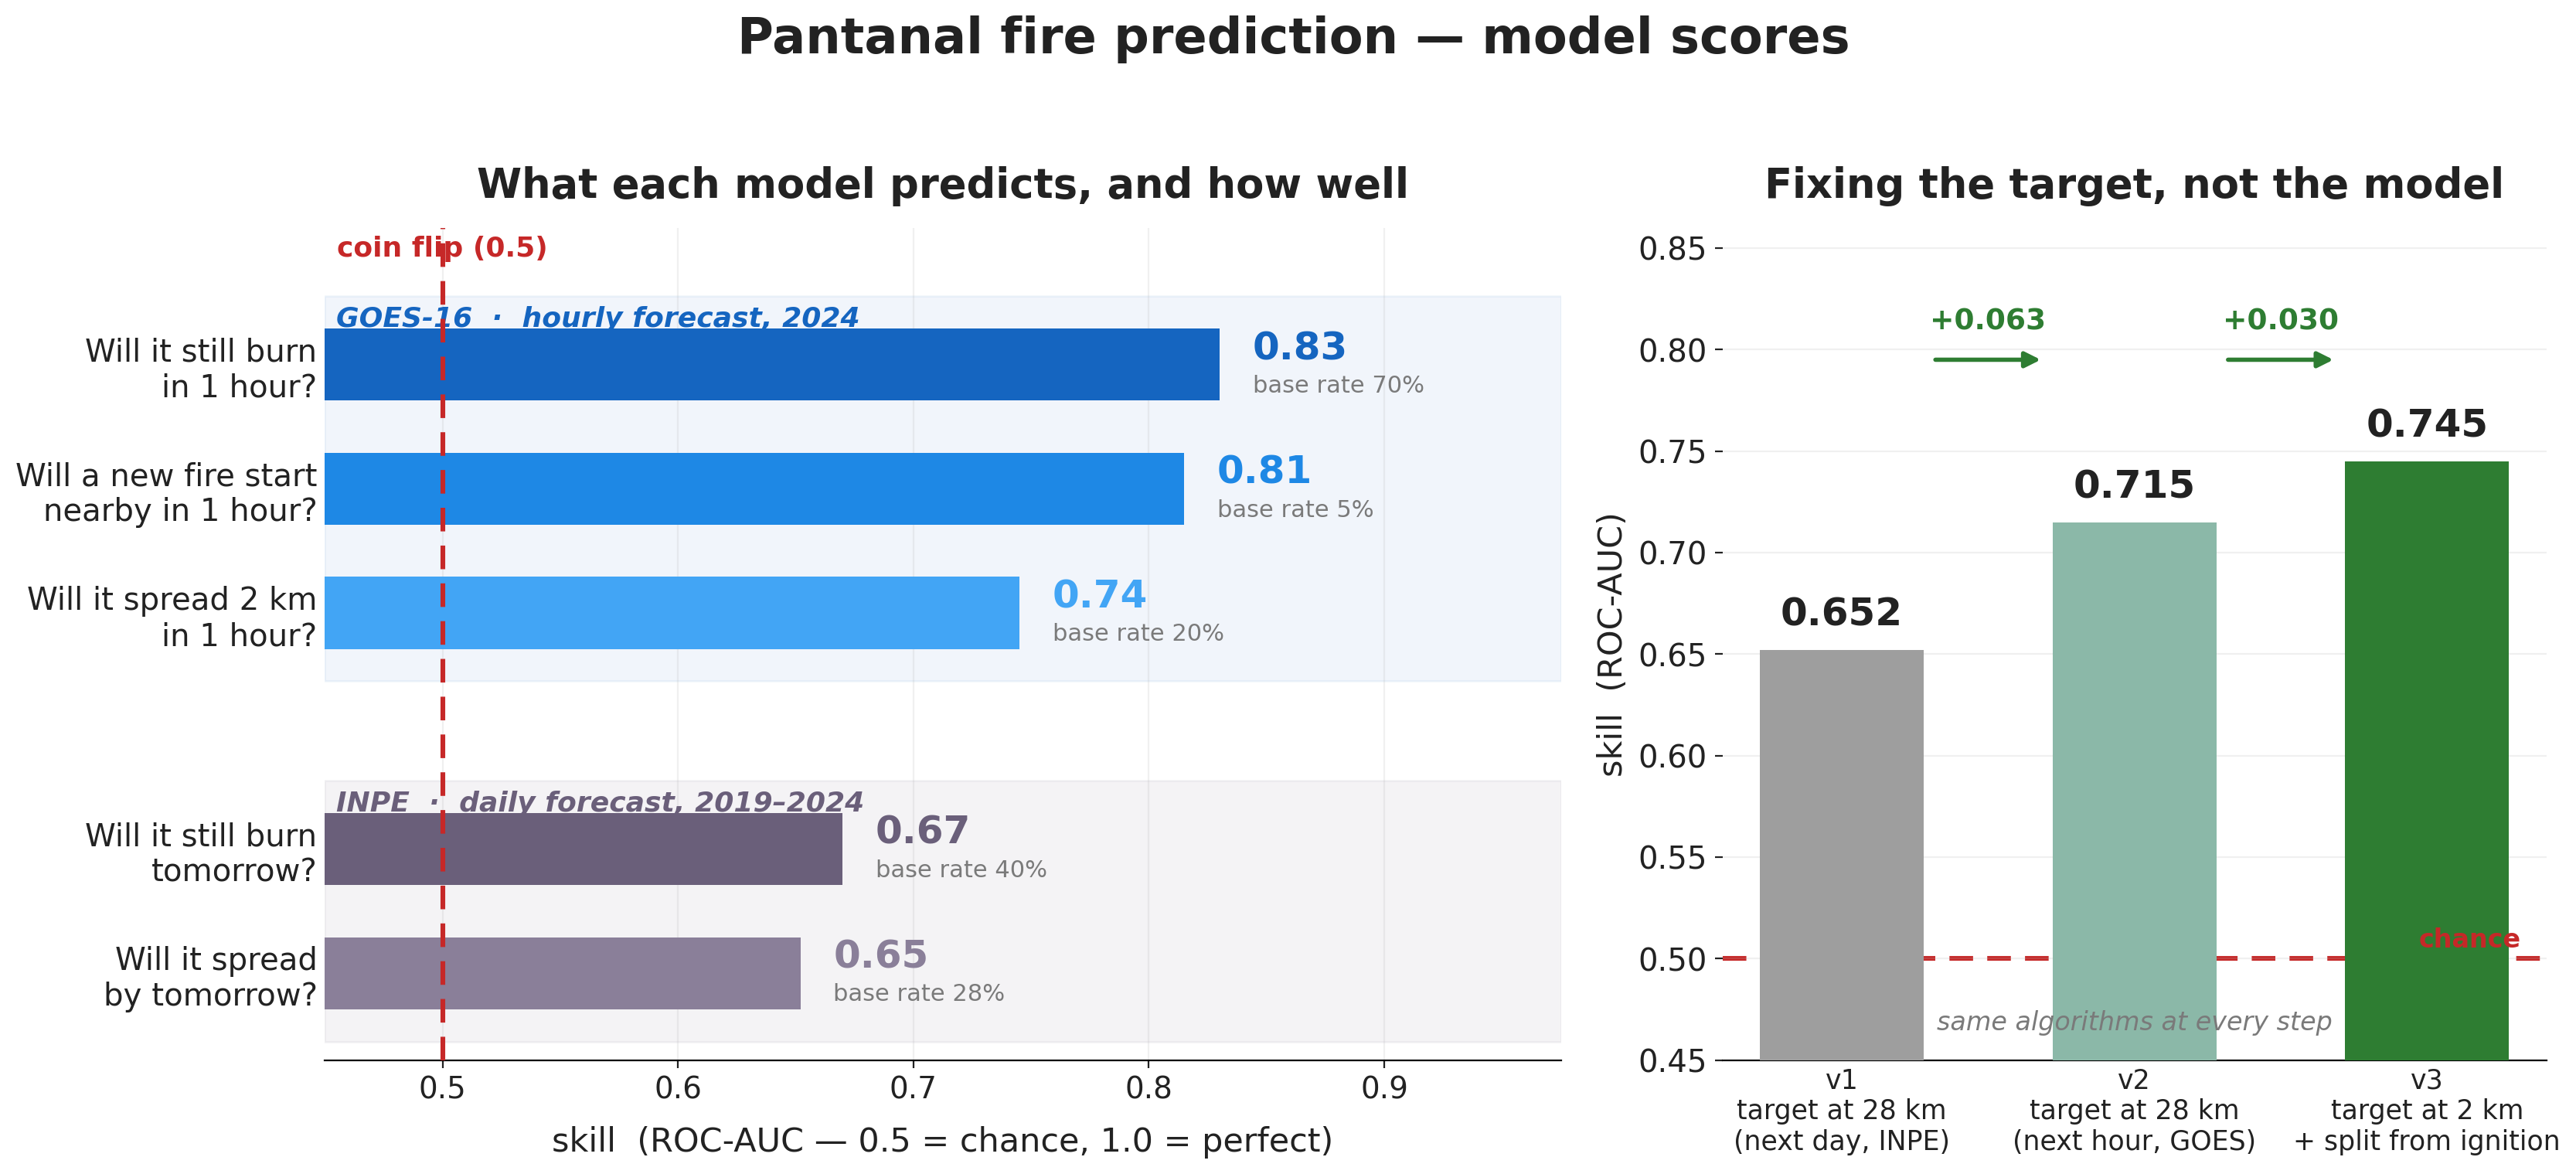
\includegraphics[width=\linewidth]{fig3_scoreboard.png}
  \caption[Model scoreboard]{\textbf{Left:} skill (ROC-AUC) of the five final
  models, with each target's base rate; the dashed line is chance.
  \textbf{Right:} progression of the spread model -- each step fixed the
  \emph{target}, not the algorithm.}
  \label{fig:scoreboard}
\end{figure}

\begin{table}[H]
\centering\small
\caption{Summary of the five final models.}
\label{tab:summary}
\begin{tabularx}{\linewidth}{>{\raggedright\arraybackslash}X l c c c}
\toprule
Question & Data & Horizon & Base rate & ROC-AUC \\
\midrule
Will this fire still burn in 1 hour? & GOES-16, 2024 & 1\,h & 70\% & \textbf{0.83} \\
Will a new fire start nearby in 1 hour? & GOES-16, 2024 & 1\,h & 5\%$^\ast$ & \textbf{0.81} \\
Will this fire spread to adjacent 2\,km ground in 1 hour? & GOES-16, 2024 & 1\,h & 20\% & \textbf{0.74} \\
Will this fire still burn tomorrow? & INPE, 2019--2024 & $\sim$24\,h & 40\% & 0.67 \\
Will fire spread around it by tomorrow? & INPE, 2019--2024 & $\sim$24\,h & 28\% & 0.65 \\
\bottomrule
\multicolumn{5}{l}{\footnotesize $^\ast$ after sampling; the true hourly ignition rate is 0.39\%.}
\end{tabularx}
\end{table}

All five models have real skill. The hourly models score higher partly because
predicting one hour ahead is easier than one day ahead, and partly because GOES-16
provides a much richer description of the fire's current state.

\section{Does weather improve the forecast?}

This question was asked at every stage. The final answer uses the five monthly
folds (test June, July, August, September, October 2024) and the paired test
described in Section~\ref{sec:stats}: in each fold, the model with meteorology is
compared with the same model without it, on the same fires.

\begin{figure}[H]
  \centering
  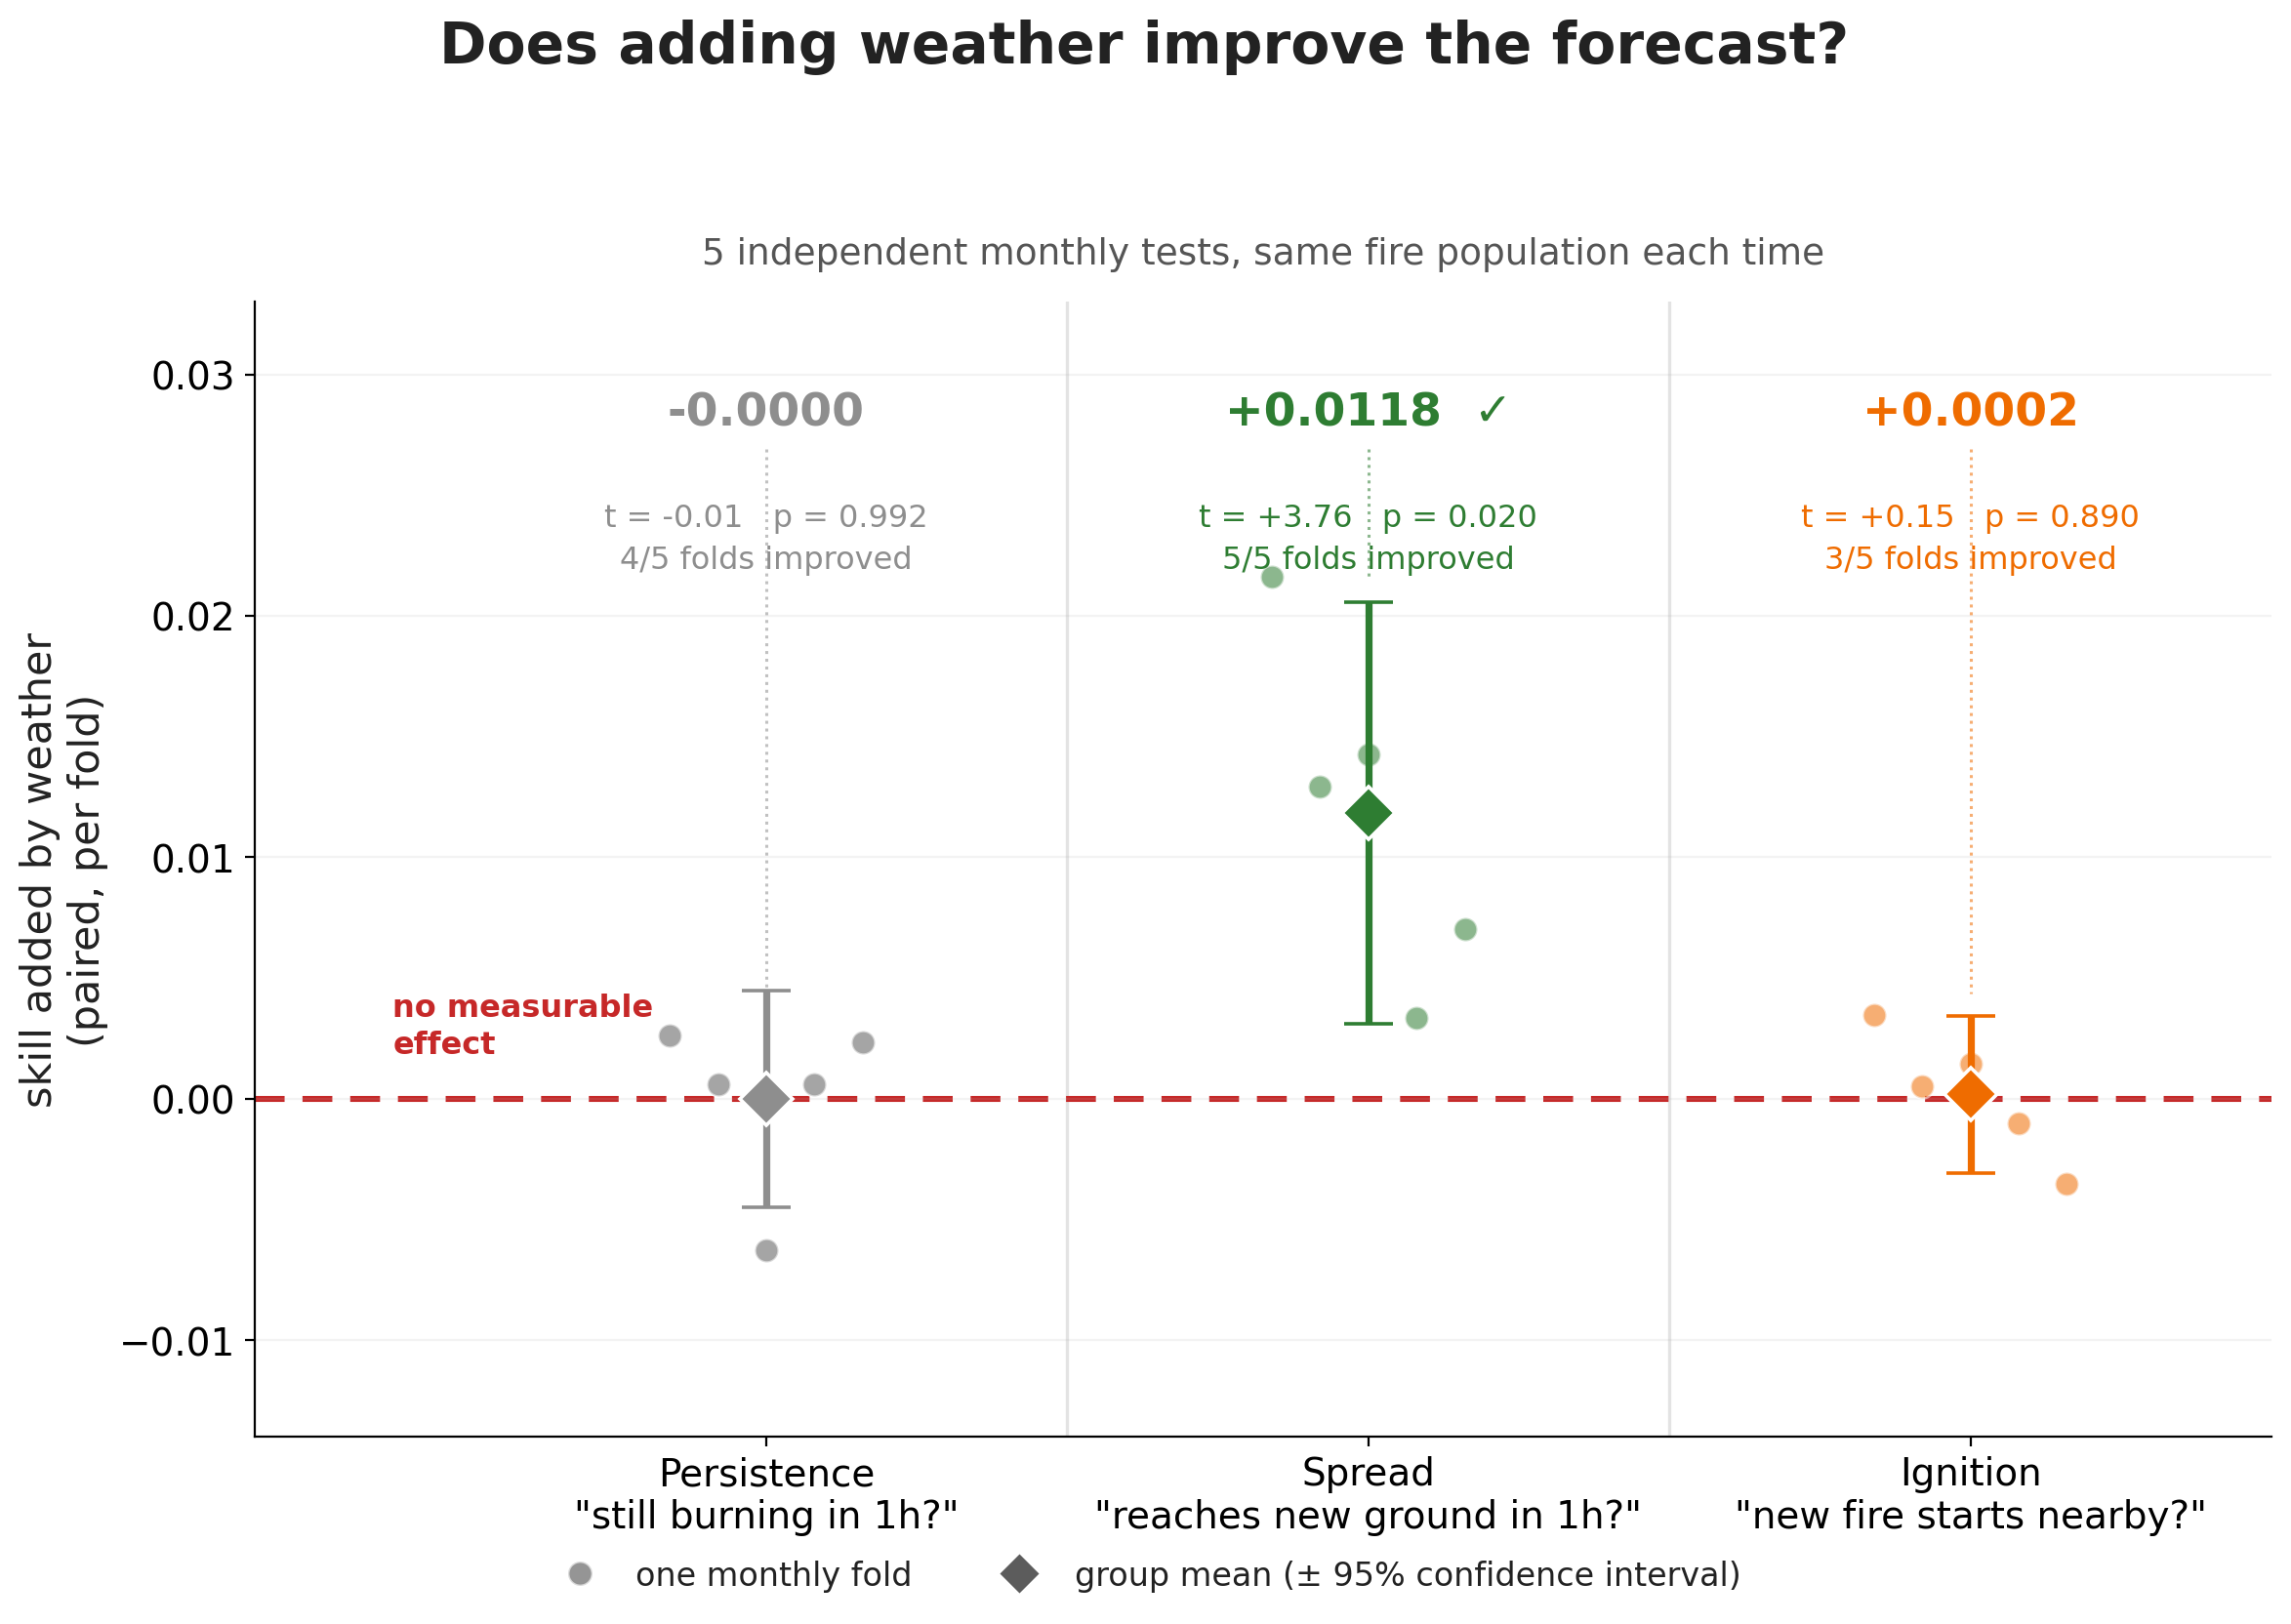
\includegraphics[width=0.88\linewidth]{fig4_weather_effect_by_target.png}
  \caption[Effect of weather on each target]{Skill added by weather features, per
  monthly fold (dots) and on average with 95\% confidence interval (diamonds and
  bars). Persistence and ignition are measured in ROC-AUC, spread in PR-AUC.}
  \label{fig:weather}
\end{figure}

\begin{table}[H]
\centering\small
\caption{Paired test of the weather block, five monthly folds.}
\label{tab:paired}
\begin{tabular}{lccccc}
\toprule
Target & Mean gain & $t$ & $p$ & Folds improved & Verdict \\
\midrule
Persistence (1\,h) & $-$0.0000 & $-$0.01 & 0.992 & 4/5 & no measurable effect \\
\textbf{Spread (2\,km)} & \textbf{+0.0118} & \textbf{+3.76} & \textbf{0.020} & \textbf{5/5} & \textbf{weather helps} \\
Ignition & +0.0002 & +0.15 & 0.890 & 3/5 & no measurable effect \\
\midrule
\textit{Spread, old 28\,km target} & \textit{+0.0053} & \textit{+2.14} & \textit{$\approx$0.10} & \textit{4/5} & \textit{suggestive only} \\
\bottomrule
\end{tabular}
\end{table}

\begin{keybox}[Key result: weather matters for spread, and only for spread]
Adding weather improves the spread forecast in every one of the five months. For
persistence and ignition, the effect is indistinguishable from zero. Fixing the
spread target roughly doubled the measured weather effect (from +0.005 to +0.012)
and made it clear -- on the old 28\,km target it was hidden.
\end{keybox}

\paragraph{How strong is the evidence?} $p=0.020$ is below the usual 0.05
threshold. Because three targets were tested, a strict statistician would apply
the \emph{Bonferroni correction} and require $p<0.05/3=0.0167$; by that standard
the result is just short of conclusive. It is supported, however, by independent
physical evidence (Figure~\ref{fig:mechanism}) and by its consistency (5 of 5
folds). Note also that the folds share part of their training data, so they are
not fully independent; the test should be read as strong but not definitive.
More years of data would settle it.

\section{Why: the physical mechanisms}

\begin{figure}[H]
  \centering
  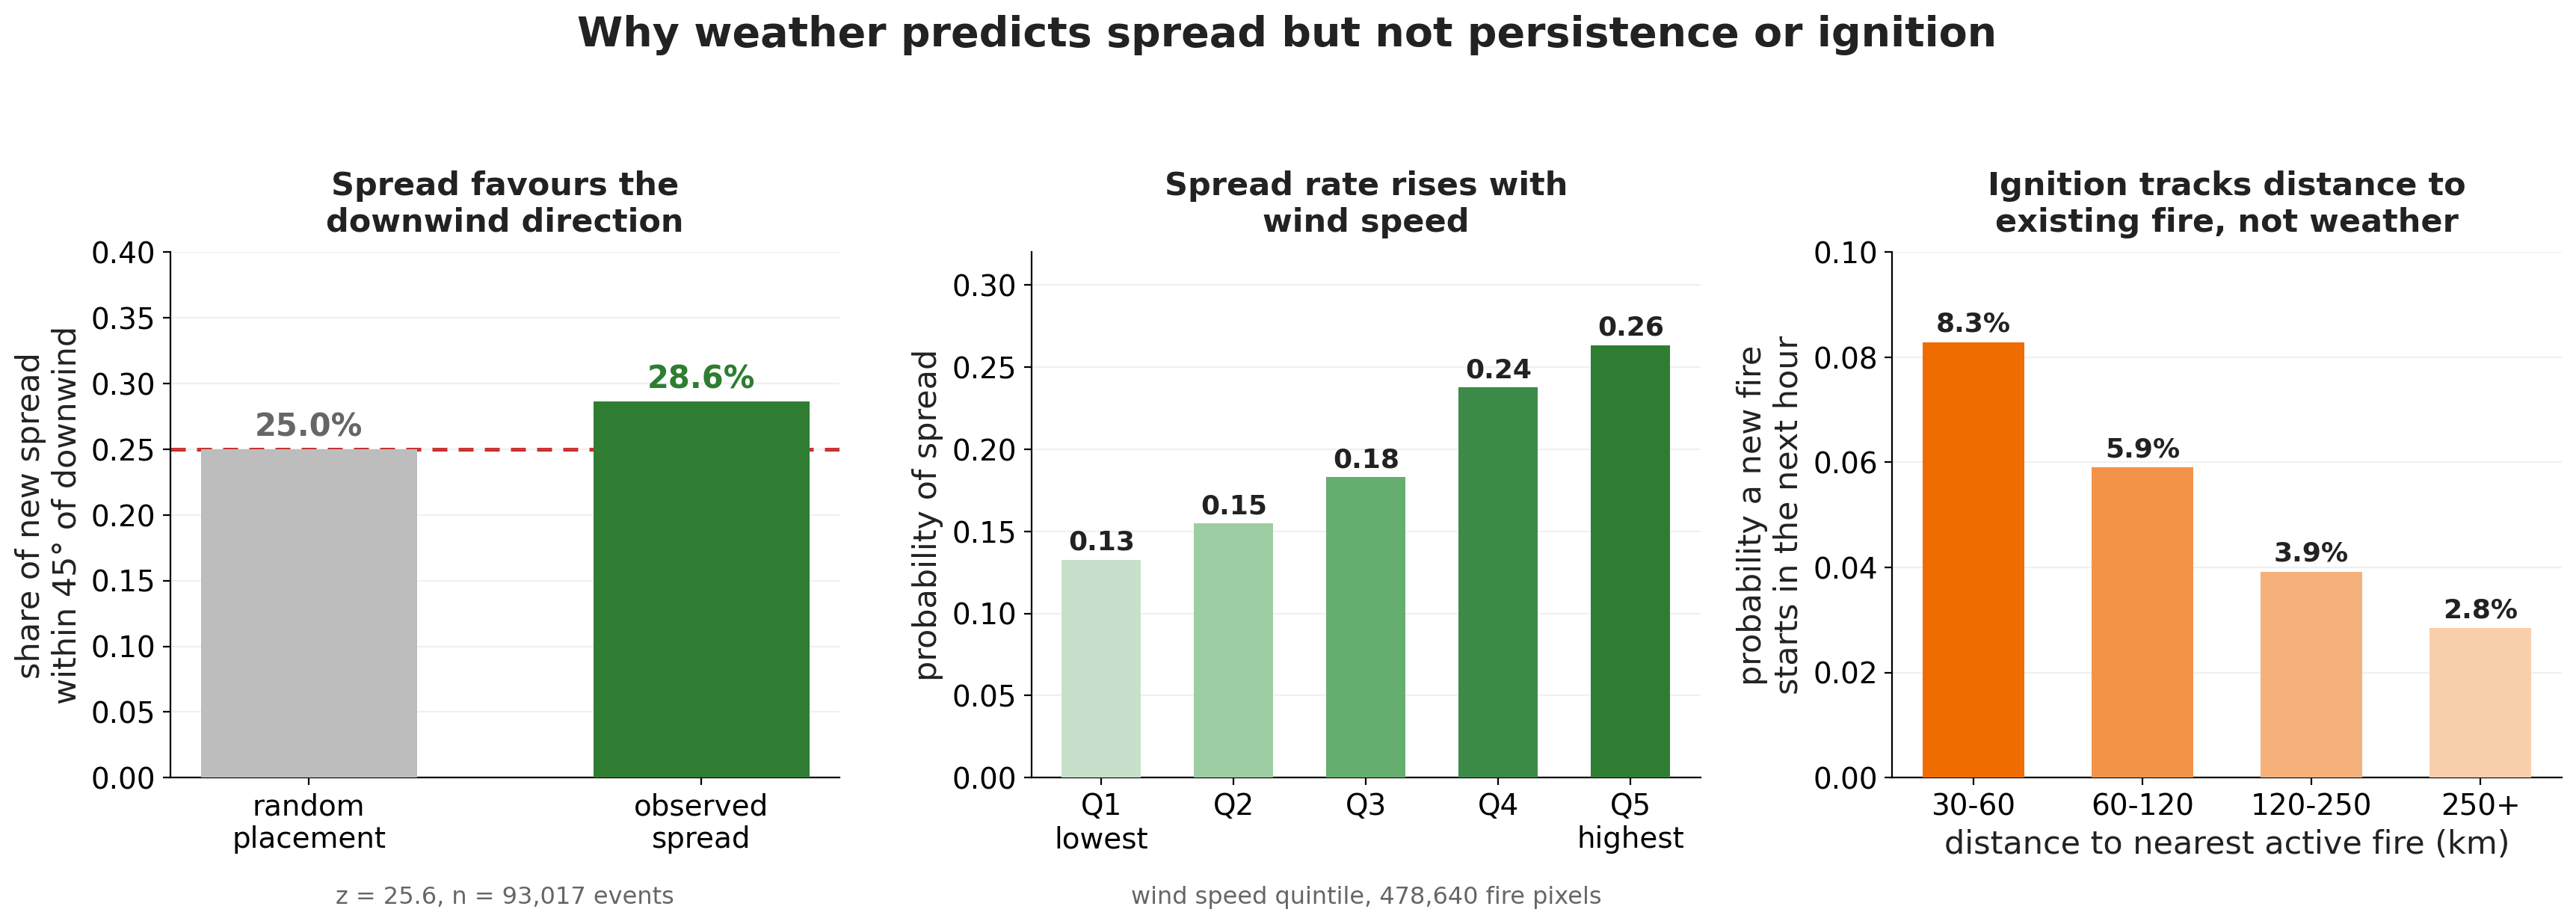
\includegraphics[width=\linewidth]{fig5_spread_mechanism.png}
  \caption[Physical mechanisms behind the result]{\textbf{Left:} new fire pixels
  appear downwind more often than at random. \textbf{Centre:} the probability of
  spread rises steadily with wind speed. \textbf{Right:} ignition probability falls
  with distance to the nearest active fire (first bin: under 60\,km; rates on the
  sampled table, 2024).}
  \label{fig:mechanism}
\end{figure}

\begin{description}
  \item[Persistence -- the fire's momentum.] Whether a fire is still burning in
        one hour is almost entirely determined by what it is doing now: its size,
        its power, how long it has been burning. The weather does not change
        enough within an hour to overturn that. (At the 24\,h horizon of the INPE
        model, by contrast, hourly wind \emph{did} help persistence, at 3.4\sig:
        over a day, weather has time to act.)
  \item[Spread -- wind and dryness.] Fire advancing into unburnt vegetation is
        exactly the process that wind and dry air control. The data show it
        directly: spread favours the downwind direction, and the spread rate
        doubles from the calmest to the windiest fifth of cases (0.13 to 0.26).
  \item[Ignition -- people and proximity.] New fires appear close to existing
        fire activity: the ignition rate falls from 8.3\% within 60\,km of an
        active fire to 2.8\% beyond 250\,km, and more than half of ignitions occur
        in cells that burned during the previous day. This is the signature of
        human ignition (burning spreading along the same roads, farms and
        land-clearing fronts) and of fires flaring up again, not of weather
        creating fires. In a region where most fires are started by people, this
        is the expected result.
\end{description}

\begin{plainbox}[Interpreting \enquote{no effect} correctly]
\enquote{Weather adds nothing to the ignition forecast} does \emph{not} mean
\enquote{weather has nothing to do with fire}. It means: once we already know
where fire is active right now, knowing the weather adds no further
\emph{hour-scale} information. Weather certainly shapes the fire season as a
whole -- the dry season is why there is fire at all -- but that information is
already contained in the current fire activity and in the season features.
\end{plainbox}

% =====================================================================
\chapter{Limitations}\label{ch:limits}
% =====================================================================

\begin{itemize}
  \item \textbf{One year of GOES-16 data.} All hourly models use 2024 only, a
        severe year. The INPE experience showed that one year cannot capture
        differences between years; the hourly results need confirming on
        2020--2024.
  \item \textbf{Folds cover the fire season only.} The monthly folds run from June
        to October; nothing is tested on wet-season-only conditions.
  \item \textbf{Different study areas.} The GOES models cover the Pantanal and its
        surroundings (including Bolivia and Paraguay), the INPE models the
        Brazilian Pantanal biome only. Their scores are not directly comparable.
  \item \textbf{Weather at 28\,km for fire at 2\,km.} ERA5 describes the average
        weather over a 28\,km cell. Local winds around a fire are not resolved, so
        the weather effect on spread is probably \emph{under}-estimated.
  \item \textbf{One scan per hour.} GOES-16 scans every 10 minutes, but one scan
        per hour was used to limit the download. Fires shorter than an hour can
        be missed.
  \item \textbf{Missing drivers.} Fuel load, land use, soil moisture, rainfall,
        flooding extent and human activity (roads, farms, firefighting) are not in
        the data, although they are known to control fire.
  \item \textbf{Satellite detection is not ground truth.} Clouds, smoke and pixel
        size all affect what is detected; part of what is labelled
        \enquote{ignition} is re-detection of an existing fire.
  \item \textbf{Weather significance is strong but not definitive}
        ($p=0.020$, above the strict Bonferroni threshold of 0.0167).
  \item \textbf{Daily model issues not fixed at source.} The filtering artefact,
        the unseeded tuning and the possible wind-direction inversion were
        identified in the laboratory's daily notebook but that notebook was not
        rebuilt.
\end{itemize}

% =====================================================================
\chapter{Conclusion and future work}\label{ch:conclusion}
% =====================================================================

\section{Conclusion}

This internship set out to build an hourly version of the laboratory's daily fire
model for the Pantanal. It ended with five working models, a validated hourly
fire record from a geostationary satellite, and a clear answer to the question of
where weather matters.

The main lessons are:
\begin{enumerate}
  \item \textbf{The target matters more than the algorithm.} The same algorithms
        were used throughout. The spread model improved from ROC-AUC 0.652 to
        0.715 to 0.745 because the \emph{question} was made more precise -- first
        hourly, then at the right spatial scale, then separated from ignition.
  \item \textbf{The observing system defines what can be predicted.} A satellite
        passing once a day cannot support an hourly forecast, whatever the time
        stamps suggest. GOES-16 made the hourly target possible and revealed a
        strong daily fire cycle, including night-time activity invisible to INPE.
  \item \textbf{Weather controls spread, not persistence or ignition, at the
        one-hour scale.} Persistence follows the fire's own momentum, ignition
        follows existing (mostly human) fire activity, and spread follows wind and
        dryness.
  \item \textbf{Honest evaluation is most of the work.} Filtering artefacts,
        leaking features, unseeded tuning, silently missing data and
        misinterpreted importances would each have produced convincing but wrong
        numbers. Checking every surprising result against physics and against
        noise was what made the final numbers trustworthy.
\end{enumerate}

\section{Future work}

\begin{itemize}
  \item \textbf{More years.} Extend GOES-16 to 2020--2024 (about 44{,}600 files,
        $\sim$76\,GB, a few hours of download). This would test the weather effect
        across contrasting years and settle its significance. GOES-19 has since
        replaced GOES-16 as the operational GOES-East satellite, so going beyond
        early 2025 means switching satellite (same product format).
  \item \textbf{Restrict to the biome}, and compare the Pantanal with the
        surrounding Cerrado.
  \item \textbf{Predict direction}, not only whether spread happens: the native
        pixel store already records where fire goes.
  \item \textbf{Longer horizons.} Train the GOES models at 3, 6, 12 and 24\,h to
        find the horizon at which weather starts to matter for persistence (it
        does not at 1\,h, and does at 24\,h).
  \item \textbf{New drivers:} soil moisture, rainfall, flooded area, vegetation
        dryness, ENSO state, and XHWI once it covers several years.
  \item \textbf{Human versus climate ignition:} separate re-detections from true
        new starts and add land-use and road-distance data.
  \item \textbf{Six scans per hour} to catch short-lived fires.
  \item \textbf{Fix the daily model} at source: rebuild its table without the
        two-day filter, seed its tuning and confirm its wind convention.
\end{itemize}

\section{Personal contribution and skills developed}

During this internship I designed and implemented the full pipeline described in
this report: data download and processing for three satellite and reanalysis
sources, construction of the fire events and targets, feature engineering,
model training and tuning, statistical evaluation, and the figures. The work
developed skills directly relevant to industrial engineering and data-driven
decision making:
\begin{itemize}
  \item handling large, messy, real-world datasets (tens of thousands of files,
        gigabytes of gridded data, missing and corrupted records);
  \item building reproducible, time-aware machine-learning experiments;
  \item statistical reasoning: noise floors, effect sizes, paired tests, and the
        difference between \enquote{not significant} and \enquote{no effect};
  \item critically auditing results, including an existing model, and
        communicating them to a scientific audience from another field
        (meteorology).
\end{itemize}

% =====================================================================
\appendix
% =====================================================================

\chapter{Feature dictionary}\label{app:features}

\section{INPE-based model (77 features)}

\begin{table}[H]
\centering\small
\caption{INPE-based model features.}
\begin{tabularx}{\linewidth}{>{\raggedright\arraybackslash}p{3.2cm} >{\raggedright\arraybackslash}X}
\toprule
Block & Features \\
\midrule
Baseline (27) & \code{lat}, \code{lon}, \code{n\_hotspots}, \code{persistence\_accumulated}
(days already burning), seasonal sine/cosine of day of year and month,
\code{year}; daily ERA5 mean/max of temperature, RH, VPD and wind speed;
atmospheric blocking counts (total, north, south, with 1--2 day lags); SACZ
indicators. \\
\addlinespace
Hourly thermal (26) & temperature, RH and VPD at detection time and 1--12\,h
before; 24\,h max/mean/min and previous-12\,h minimum; hours above 32 and
35\,$^\circ$C, hours with RH below 30\%, hours with VPD above 20\,hPa. \\
\addlinespace
Geometry (11) & cluster spread, radius, elongation and axis orientation; distance
to nearest same-day fire; number of fires in the 5--20\,km ring; movement since
the previous overpass. \\
\addlinespace
Hourly wind (13) & wind speed now and 3--12\,h before, 24\,h max/mean,
previous-12\,h minimum, direction variability, $u$/$v$ components, direction
(sine/cosine), wind--movement alignment. \\
\addlinespace
Timing (excluded) & detection hour, time to next overpass -- dropped after testing
(Section~\ref{sec:timing}). \\
\addlinespace
XHWI (conditional) & 13 heatwave-index features; used only if available for every
year (currently 2024 only). \\
\bottomrule
\end{tabularx}
\end{table}

\section{GOES-16 models}

\begin{table}[H]
\centering\small
\caption{GOES-16 model features.}
\begin{tabularx}{\linewidth}{>{\raggedright\arraybackslash}p{3.2cm} >{\raggedright\arraybackslash}X}
\toprule
Block & Features \\
\midrule
Context (all models) & \code{lat}, \code{lon}, hour of day (sine/cosine), day of
year (sine/cosine). \\
\addlinespace
Fire state (persistence, 28\,km) & number of fire pixels, fire area (km$^2$),
fraction of cell burning, max and total fire radiative power, max pixel fire area
and temperature, measurement-available flags, fire present 1/2/3/6/12/24\,h ago,
hours burning in the last 6 and 24\,h, power and pixel count 1\,h ago and change,
number of neighbouring cells and pixels burning (now and 1\,h ago). \\
\addlinespace
Fire state (spread, 2\,km) & pixel fire power, area, temperature; number of
burning neighbours; size of the burning patch; fire pixels in the region; hours
burning in the last 6 and 24\,h. \\
\addlinespace
Fire activity (ignition) & distance to nearest active fire; hours the cell burned
in the last 24\,h; number of burning cells in the region. \\
\addlinespace
Meteorology & temperature, RH, VPD, wind speed (and for the 28\,km and spread
models $u$/$v$ wind components); the 28\,km model also uses 1--12\,h lags and
24\,h max/mean/min. \\
\addlinespace
Excluded (leakage) & spread bearing, downwind flag, wind--spread angle (describe
the outcome). \\
\bottomrule
\end{tabularx}
\end{table}

\chapter{Detailed fold results}

\begin{table}[H]
\centering\small
\caption{Rolling-origin folds, 2\,km spread (PR-AUC) and ignition (ROC-AUC).}
\begin{tabular}{lcccccc}
\toprule
 & \multicolumn{3}{c}{Spread 2\,km} & \multicolumn{3}{c}{Ignition} \\
\cmidrule(lr){2-4}\cmidrule(lr){5-7}
Test month & context & + fire & + met & context & + activity & + met \\
\midrule
June      & 0.2979 & 0.3563 & 0.3779 & 0.6734 & 0.8231 & 0.8266 \\
July      & 0.3041 & 0.3963 & 0.4093 & 0.6997 & 0.8414 & 0.8419 \\
August    & 0.3778 & 0.4257 & 0.4400 & 0.6124 & 0.8697 & 0.8712 \\
September & 0.3742 & 0.4361 & 0.4394 & 0.6826 & 0.8777 & 0.8767 \\
October   & 0.3391 & 0.4052 & 0.4122 & 0.6543 & 0.7941 & 0.7906 \\
\bottomrule
\end{tabular}
\end{table}

\begin{table}[H]
\centering\small
\caption{Rolling-origin folds, 28\,km model: persistence (ROC-AUC) and spread (PR-AUC).}
\begin{tabular}{lcccccc}
\toprule
 & \multicolumn{3}{c}{Persistence 1\,h} & \multicolumn{3}{c}{Spread 28\,km} \\
\cmidrule(lr){2-4}\cmidrule(lr){5-7}
Test month & context & + fire & + met & context & + fire & + met \\
\midrule
June      & 0.6334 & 0.7913 & 0.7939 & 0.2452 & 0.2817 & 0.2814 \\
July      & 0.6780 & 0.8084 & 0.8090 & 0.2452 & 0.2937 & 0.3047 \\
August    & 0.6358 & 0.8065 & 0.8002 & 0.3464 & 0.3987 & 0.4030 \\
September & 0.6309 & 0.8198 & 0.8204 & 0.3646 & 0.4184 & 0.4189 \\
October   & 0.6321 & 0.8280 & 0.8303 & 0.3319 & 0.3671 & 0.3781 \\
\midrule
Mean      & 0.6420 & 0.8108 & 0.8108 & 0.3066 & 0.3519 & 0.3572 \\
\bottomrule
\end{tabular}
\end{table}

\begin{table}[H]
\centering\small
\caption{GOES-16 fire activity by month, 2024 (28\,km table).}
\begin{tabular}{lrcc@{\hspace{1.2cm}}lrcc}
\toprule
Month & Rows & Persists & Spreads & Month & Rows & Persists & Spreads \\
\midrule
Jan & 6{,}134 & 0.513 & 0.154 & Jul & 9{,}629 & 0.680 & 0.173 \\
Feb & 4{,}500 & 0.446 & 0.230 & Aug & 32{,}622 & 0.747 & 0.237 \\
Mar & 7{,}617 & 0.495 & 0.263 & Sep & 30{,}787 & 0.753 & 0.223 \\
Apr & 2{,}885 & 0.531 & 0.094 & Oct & 12{,}003 & 0.657 & 0.217 \\
May & 5{,}398 & 0.627 & 0.095 & Nov & 3{,}989 & 0.537 & 0.180 \\
Jun & 12{,}726 & 0.697 & 0.184 & Dec & 2{,}260 & 0.477 & 0.145 \\
\bottomrule
\end{tabular}
\end{table}

\chapter{Problems found and fixed}

\begin{table}[H]
\centering\small
\caption{Data and code problems found during the project.}
\label{tab:bugs}
\begin{tabularx}{\linewidth}{>{\raggedright\arraybackslash}p{3.6cm} >{\raggedright\arraybackslash}X >{\raggedright\arraybackslash}p{3.8cm}}
\toprule
Problem & Consequence & Fix \\
\midrule
Daily table keeps only fires lasting $\geq$2 days & persistence 0.93 mostly an artefact (trivial rule 0.905) & reported; hourly table unfiltered \\
Unseeded Optuna search & identical runs 0.631 vs 0.601 & seeded sampler; multi-seed tests \\
Time-to-next-overpass from Pantanal only & target leak (0.218 vs 0.477) & regional overpass time, then dropped \\
Heatwave \enquote{hours since peak} on all-zero windows & calm confused with decayed & sentinel value $-1$ \\
Biome filter before observation test & 433 instead of 76 clusters wrongly dropped & scope by state first \\
Fire chains crossing the train/test cut & same fire in both sets & chains purged \\
Timing features & high importance, but hurt the model & removed \\
INPE zero-fill hourly target & hour of day alone gives ROC-AUC 0.917 & switch to GOES-16 \\
Full-disk decoding & 3.3\,s per file & windowed HDF5 read, 83\,ms \\
Network drop during download & April 2024 silently missing & retries with backoff \\
Lags built from observed rows & 1-h lag reached 2\,h back ($\sim$1.6\% of hours) & complete hourly time axis \\
Missing fire power stored as 0 & model learned a measurement flag & keep missing + flags \\
28\,km spread target & not physical (7.7\,m/s, random direction) & 2\,km pixels, split target \\
Wind direction convention (daily notebook) & alignment sign possibly inverted & store direction \enquote{to} only \\
\bottomrule
\end{tabularx}
\end{table}

\chapter{Code organisation and reproduction}

\begin{table}[H]
\centering\small
\caption{Main scripts.}
\begin{tabularx}{\linewidth}{>{\raggedright\arraybackslash}p{6.4cm} >{\raggedright\arraybackslash}X}
\toprule
File & Role \\
\midrule
\multicolumn{2}{l}{\textit{\code{hourly\_model/} -- INPE-based model}} \\
\code{build\_fire\_events\_hourly.py} & INPE detections $\rightarrow$ clusters (DBSCAN) \\
\code{download\_era5\_pantanal.py} & hourly ERA5 download (Copernicus CDS API) \\
\code{build\_hourly\_dataset.py} & fire chains, targets and hourly features \\
\code{ml\_persistence\_spread\_hourly.ipynb} & training, tuning, evaluation \\
\code{feature\_set\_effect\_size.py} & multi-seed effect-size test \\
\addlinespace
\multicolumn{2}{l}{\textit{\code{goes\_hourly\_model/} -- GOES-16 models}} \\
\code{goes\_grid.py} & GOES fixed-grid $\leftrightarrow$ latitude/longitude \\
\code{build\_goes\_hourly.py} & hourly fire mask per ERA5 cell \\
\code{validate\_goes\_vs\_inpe.py} & August 2024 validation \\
\code{build\_goes\_model\_table.py}, \code{train\_goes\_hourly.py} & 28\,km model \\
\code{build\_goes\_pixels.py} & native 2\,km fire-pixel store \\
\code{build\_goes\_split\_targets.py}, \code{train\_goes\_split.py} & spread and ignition models \\
\code{make\_*\_figures.py} & figures \\
\bottomrule
\end{tabularx}
\end{table}

Typical reproduction sequence (INPE model):
\begin{verbatim}
python build_fire_events_hourly.py --years 2019-2024 \
       --states "MATO GROSSO DO SUL,MATO GROSSO"
python download_era5_pantanal.py --years 2019-2024
python build_hourly_dataset.py
python feature_set_effect_size.py --seeds 5
\end{verbatim}
Downloading ERA5 requires a personal Copernicus CDS account and API key, stored
in the user's \code{.cdsapirc} file. GOES-16 data are public and need no account.

\chapter{Glossary}

\begin{description}[style=nextline,leftmargin=0.6cm,itemsep=0.35em]
\item[Base rate / prevalence] How often the predicted event happens in the data.
\item[Cross-validation] Repeatedly training on part of the data and checking on
another part, to choose settings without touching the test set.
\item[DBSCAN] A clustering method grouping points closer than a set distance.
\item[Embargo] A time gap left between training and test data to avoid the same
event appearing on both sides.
\item[ERA5] ECMWF's global hourly reanalysis of the atmosphere.
\item[Feature] An input variable given to the model.
\item[Fire radiative power (FRP)] Energy released by a fire per second, measured
from space (megawatts).
\item[Fold] One train/test round in a repeated evaluation.
\item[Geostationary satellite] A satellite that stays above the same point of the
equator and observes continuously.
\item[GOES-16] NOAA's geostationary satellite over the Americas (GOES-East).
\item[Hyperparameter] A setting of the learning algorithm chosen by the user.
\item[INPE] Brazil's National Institute for Space Research, which runs the
Programa Queimadas fire-monitoring programme.
\item[Leakage] Information about the answer hidden in the inputs.
\item[Lift] PR-AUC divided by the base rate.
\item[Noise floor] The variation of a score caused by randomness alone.
\item[p-value] Probability of a difference at least this large if there were truly
no effect.
\item[Polar-orbiting satellite] A low satellite passing over a location at fixed
times each day.
\item[PR-AUC] Area under the precision--recall curve; no-skill value = base rate.
\item[Random forest] Many decision trees trained independently and averaged.
\item[Reanalysis] A reconstruction of past weather combining observations and a
model.
\item[ROC-AUC] Probability that the model ranks a random positive case above a
random negative one; 0.5 = chance.
\item[Seed] A number fixing the randomness of a computation so it can be repeated.
\item[t-statistic] Mean difference divided by its standard error.
\item[Target] The outcome the model predicts.
\item[VPD] Vapour pressure deficit: how strongly the air draws moisture from
vegetation.
\item[XGBoost] Gradient boosting: trees trained in sequence, each correcting the
previous ones.
\item[XHWI] Extreme Heatwave Index, produced by LAMMOC/UFF.
\end{description}

\end{document}
